\section{The Tile Simulation Framework}~\label{sec:tile_simulation}

The previous chapter introduced the digital back-end as well as discussed different design choices, namely tile size, routing configurations, and the effects of the aggregator position.
Here we describe how we simulate events of interest for these different configurations.

A successful design is able to record and send loss less data for all events of interest.
In a DUNE-FD LArTPC these sources range in intensity from sub-MeV-scale radiogenic backgrounds native to the LAr to 10's of GeV scale of beam neutrinos or atmospheric neutrinos.
We consider the back-end design to be successful if and only if it provides the ability to fully capture and transmit of all collected resets from these sources.

We note that while it may be shown in the future that some resets may in fact not be needed for a reconstruction of particular events, we still assert that since Q-Pix is a novel readout, it is not yet possible to claim all scientific goals for which it may be used.
For this reason we demand that no data be lost for any reason due to the digital back-end design.

\subsection{The Tile Representation}

We model a tile (a group of digital nodes, or ASICs) based on the description given in Chapter~\ref{chap:qdb}.
A tile is then represented in software (Python 3) as a linked list of nodes which store pointers to the adjacent nodes or neighbors.

We note a distinction between the nomenclature used here. 
The term "node" refers to the simulated back-end ASIC whereas our use of "ASIC" refers to the first digital prototype.

Every node in the tile holds two FIFO objects which store local and remote data. 
The local and remote FIFOs keep track of the total number of resets or packet transactions, respectively.
If a node records a new reset the local FIFO is then written to, and the local FIFO transaction counter increases.
Similarly, the remote FIFO's transaction count is increased when a write occurs on this FIFO, which happens every time a digital node receives a packet from a neighbor node, including the aggregator node.

In the current Q-Pix digital ASIC design (see Sect.~\ref{sec:digital_fsm}) all packets sent between neighbor nodes, with the exception of broadcasts, are written on the remote FIFO.
At the beginning of a simulation step each node first checks to see if its received an interrogation request.
If the node has received a soft interrogation request (see Sect.~\ref{sec:broadcast}), and has data in its local FIFO, it will first send its data in the local FIFO, followed by the event-end packet.
If the node receives a Hard Interrogation request, the node will send local data, if any, and will send an event-end packet regardless of whether or not the local FIFO had any data.
If the node's local FIFO is empty, and it has not received an interrogation, it will check the empty status of the remote FIFO.
If the remote FIFO is not empty, this packet will be read and transmitted to its neighbors accordingly, otherwise the node remains in its idle state.

%% example local vs remote of snake
\begin{figure}
\centering
\begin{subfigure}{.5\textwidth}
  \centering
  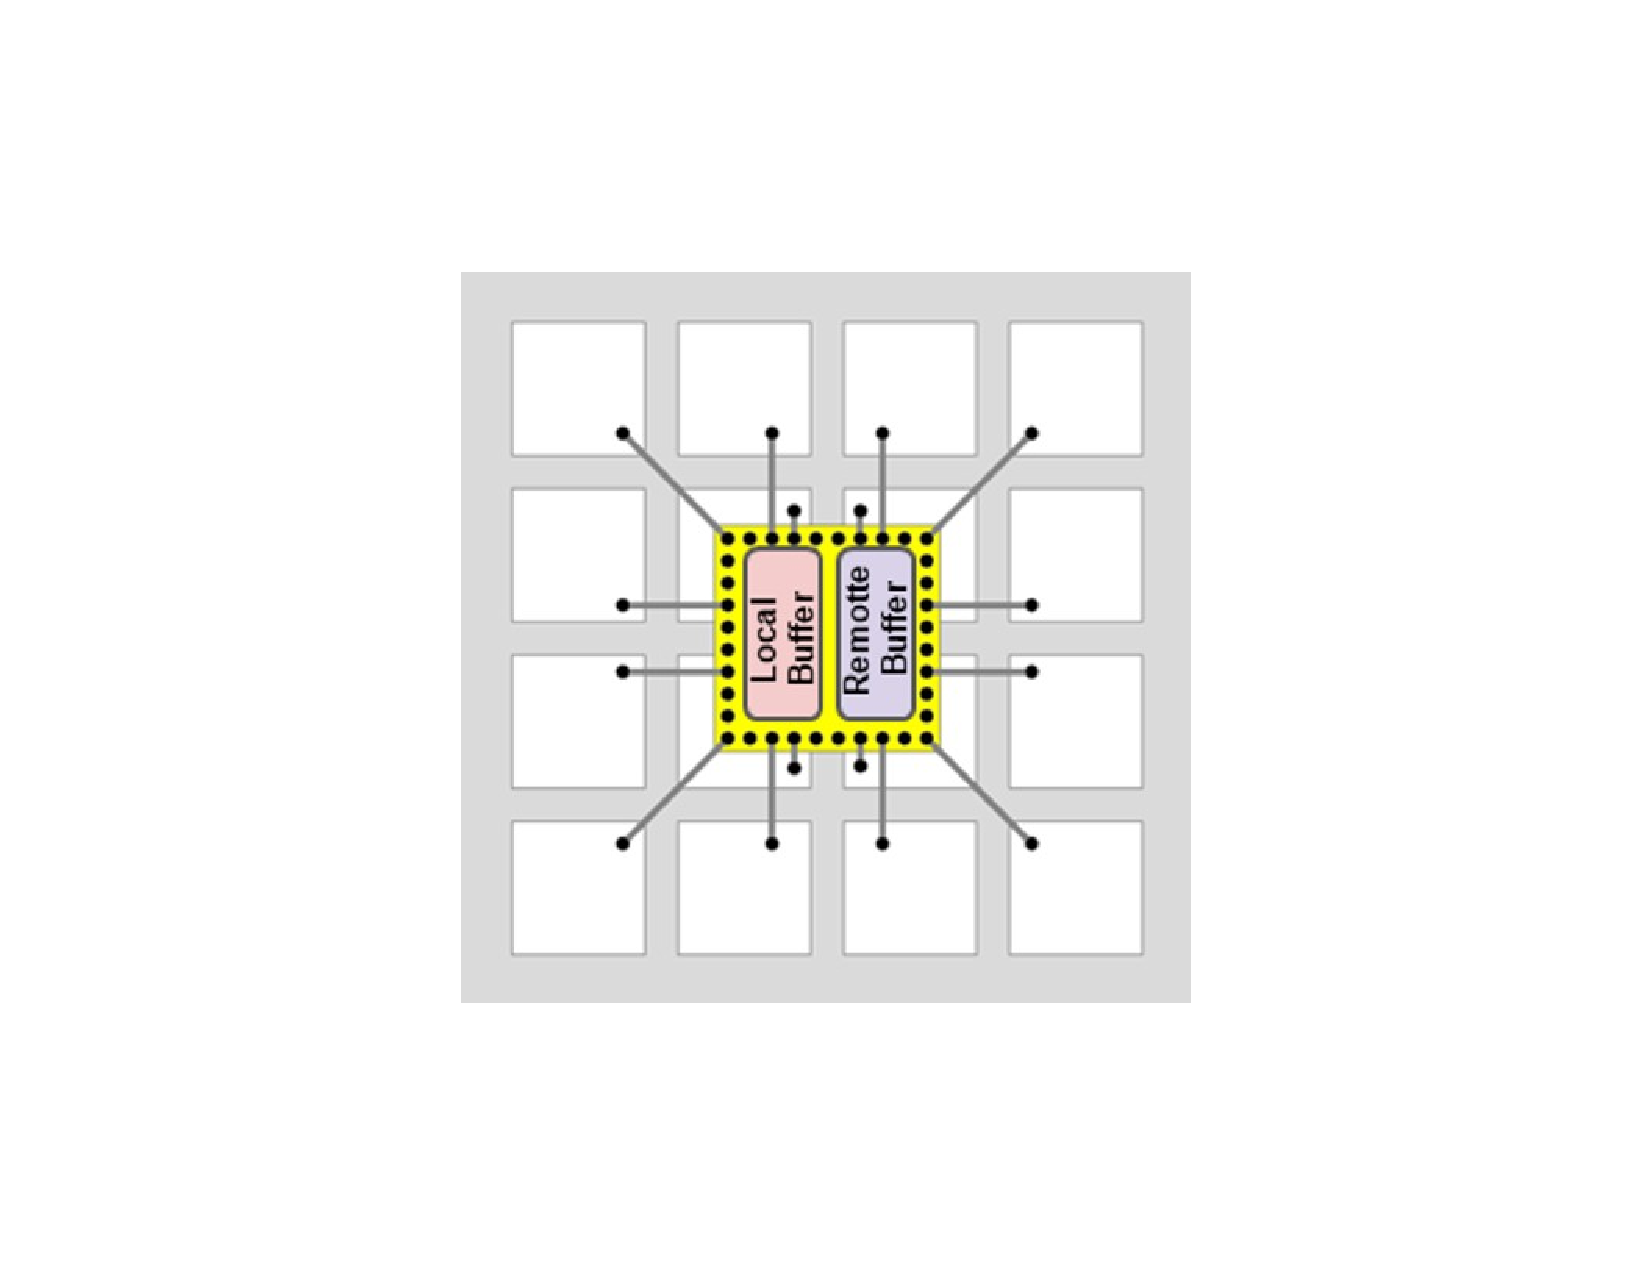
\includegraphics[width=\textwidth]{images/asic_FIFO_image.pdf}
  \caption{Individual node with local and remote FIFOs.}
\end{subfigure}%
\begin{subfigure}{.5\textwidth}
  \centering
  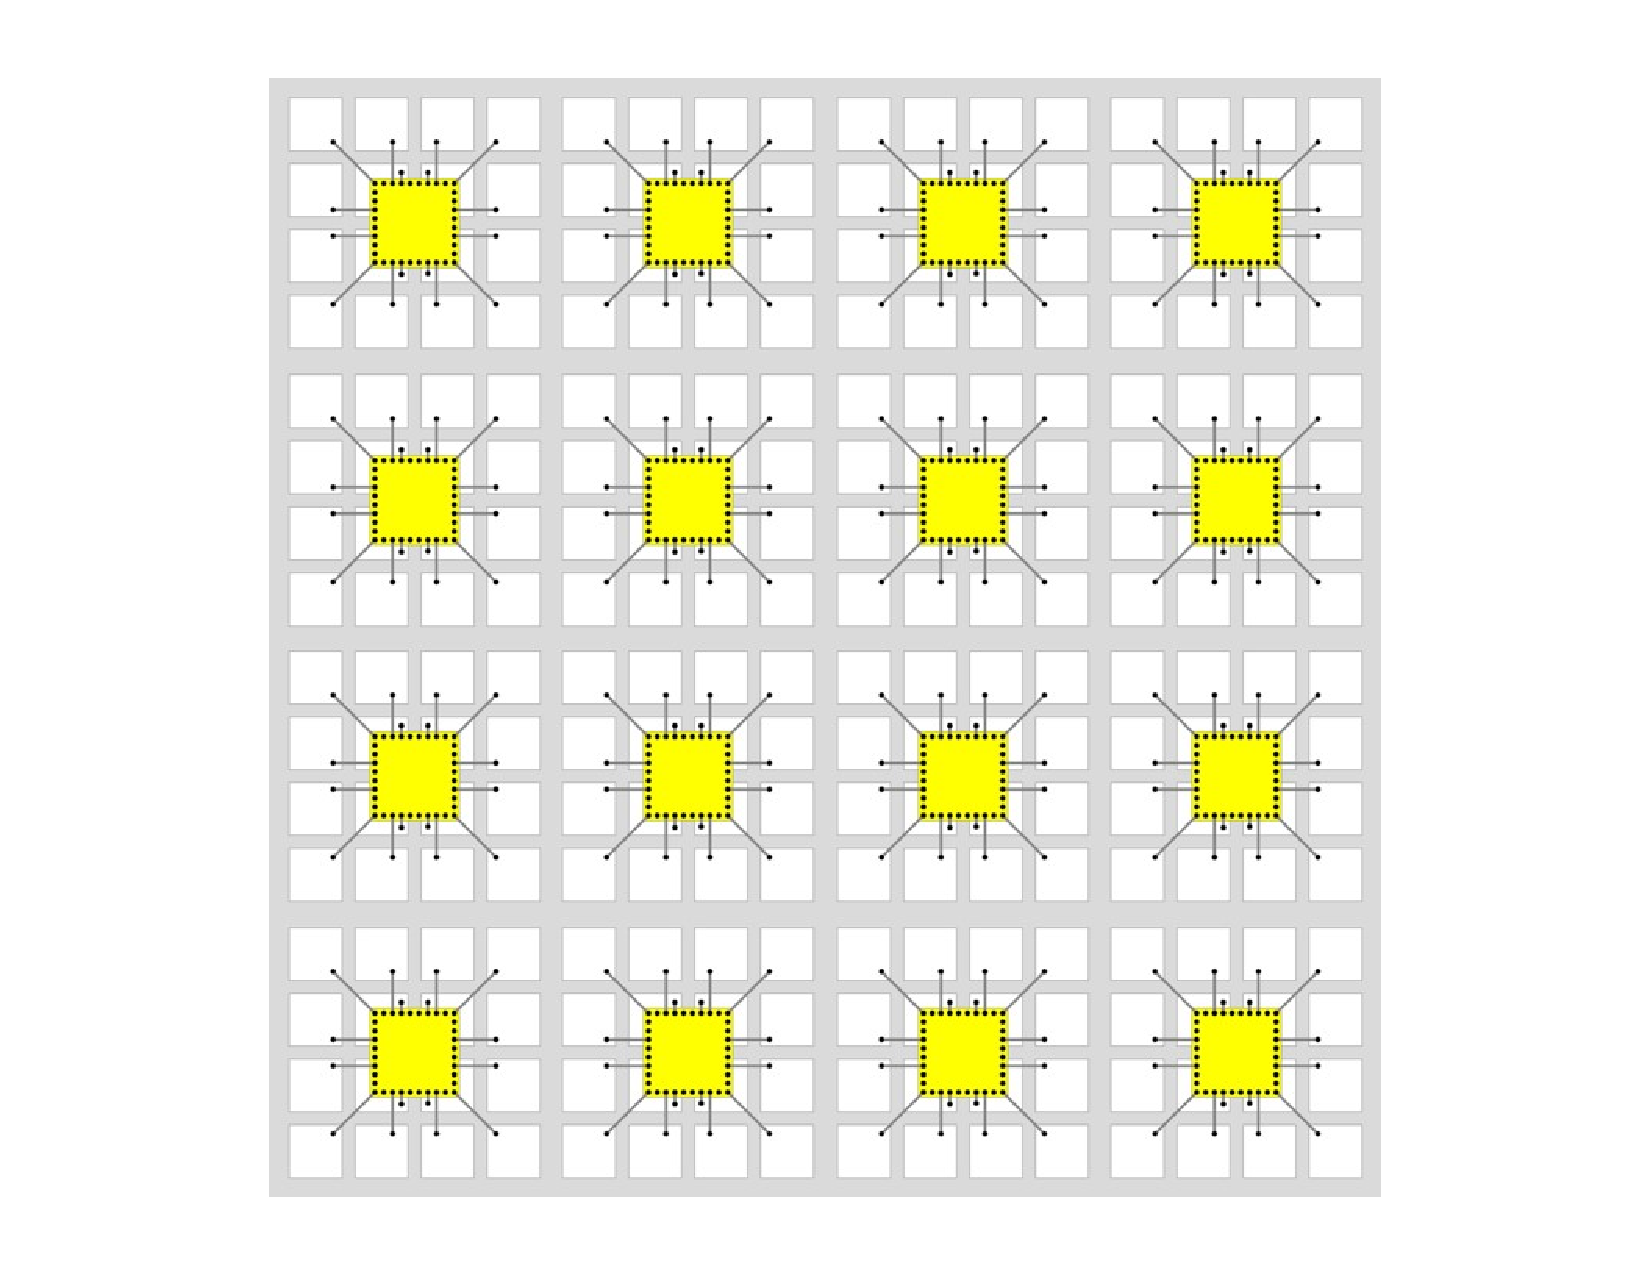
\includegraphics[width=\textwidth]{images/asic_tile_FIFO_image.pdf}
  \caption{Tile of node objects.}
\end{subfigure}
\caption{Composition of an example 4$\times$4 tile.
Each node in the tile represents a digital ASIC which contains two FIFOs.
One FIFO is used to store timestamps from reset data, which we refer to as the local FIFO.
The other FIFO we call the remote FIFO and is used to store all packet transactions from neighbor nodes.
The local FIFO is 48 bits wide, where 32 bits come from the timestamp and 16 bits are from the pixels.
The remote FIFO is 60 bits wide, since it must store all relevant bits for the 64 bit packet word, where there are 4 unused bits.
}
\label{fig:node_fifo_objects}
\end{figure}

There are two types of remote data to send: broadcasts and responses.
A broadcast is a register request sent to a digital node, which can only be created and sent from the aggregator node.
The responses include all other kinds of packets sent from neighbor nodes which include: data packets, event-end packets, and register response packets.

The communication packet object is a custom struct object which uses an enumerated type to differentiate the kinds of packets that the digital node can read from its remote FIFO.
Each simulated node's behavior to these incoming packets is mirrored to the digital FSM, shown in Fig.~\ref{fig:digital_fsm}.
When a node reads the packet from the remote FIFO it reads the enumerated type to determine how to communicate the packet to its neighbors, just as is done in the physical ASIC.

Also tested in these simulations are tiles which are have a "push" architecture.
This architecture changes the condition for a node to leave its idle state and send local data whenever the local FIFO is not empty.
For this reason the push architecture is also more time consuming to simulate since each node can send a packet at any time, provided that it will inject a hit into its local FIFO following the procedure described in the next section.
Nodes which require an interrogation in order to send local data we refer to as the "pull" architecture.

\subsection{Injected Resets}~\label{sec:hits}

In order to speed up the execution of the python simulation reset events are precalculated and loaded into separate list containers for each node.
At the beginning of every simulation time step every node checks its injected resets list against the new simulation step time.
If the new time step is larger than any of the timestamps in its resets list, the resets are then removed from this list and are written to the node's local FIFO.

Resets from simulated data whether radiogenic or neutrino data can occur at any pixel and at any time.
The digital node (and the ASIC) is capable of recording multiple resets from multiple channels at the same time.
This means that it is possible for multiple different pixel resets to only contribute to one local FIFO write.
Therefore, extra care must taken when adding injected resets with channel information.

In this simulation we consider the best case timestamp measurement for each reset, which is that each digital node can record a unique reset for each channel on every new clock cycle. 
Then, procedure for combining resets from multiple channels calculates the clock cycle (timestamp) for which this node would record a timestamp for a particular channel.
If a reset has already been recorded for this channel, the un-injected timestamp is incremented by one clock period for this node.
The above procedure then repeats until all channels have had all of their resets recorded on unique timestamps for the digital node, where only different channels can be recorded on the same timestamp.

\begin{figure}[]
\centering
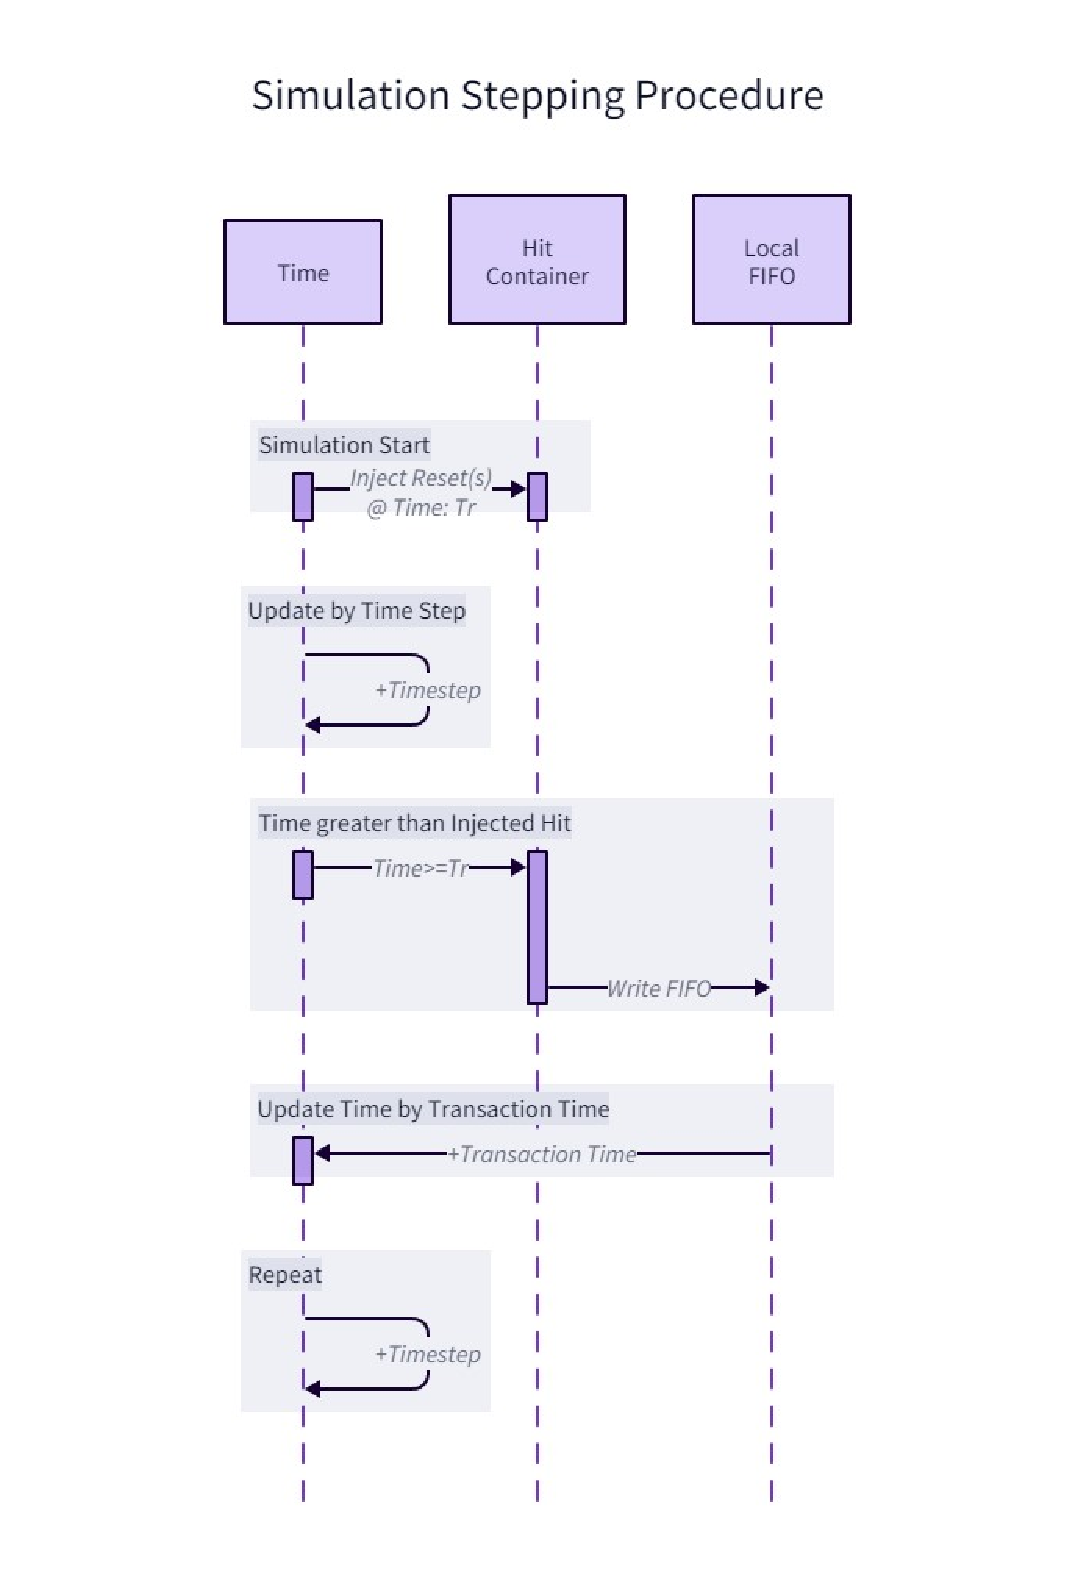
\includegraphics[width=0.7\textwidth]{images/simulation_step_procedure.pdf}
\caption{Example timeline for simulation time steps and injected hits.
Before the simulation begins hits are added into a Hit Container for each node.
When the simulation begins the time is incremented by a single time step ($\tau = 1 \mu$\unit{s}).
The time increments until it is larger than the time of any of the injected hits.
The values of the timestamps are then moved from the Hits container into the local FIFO, where the timestamp that is recorded is the soonest clock cycle after the "true" time of the injected hit.
When the data are ready to be transmitted from the local FIFO, the time is then updated by transaction time.
An example of this procedure is shown in Figure~\ref{fig:push_arch_verification}. 
}
\end{figure}~\label{fig:simulation_step_procedure}

\subsection{The Simulation Procedure}~\label{sec:process}

Upcoming sections will discuss values derived from simulating the readout of the tile. 
Here we briefly describe the simulation procedure and how the results are obtained.
The procedure is also graphically demonstrated in Figure~\ref{fig:simulation_process_procedure}.

The simulation loop iteratively processes a single transaction from a queue of transactions and then processes all nodes in the tile at incremental timestamps.
The timesteps used in the simulation results used here are steps 1~\unit{\mu s}.
It is not necessary to perform smaller time steps than this, as packet transactions themselves are on the order of $\approx 50 \unit{\mu s}$, based on the endeavor protocol.
If any processed node generates a new transaction(s), this transaction(s) is added to the transaction queue.

\begin{figure}[]
\centering
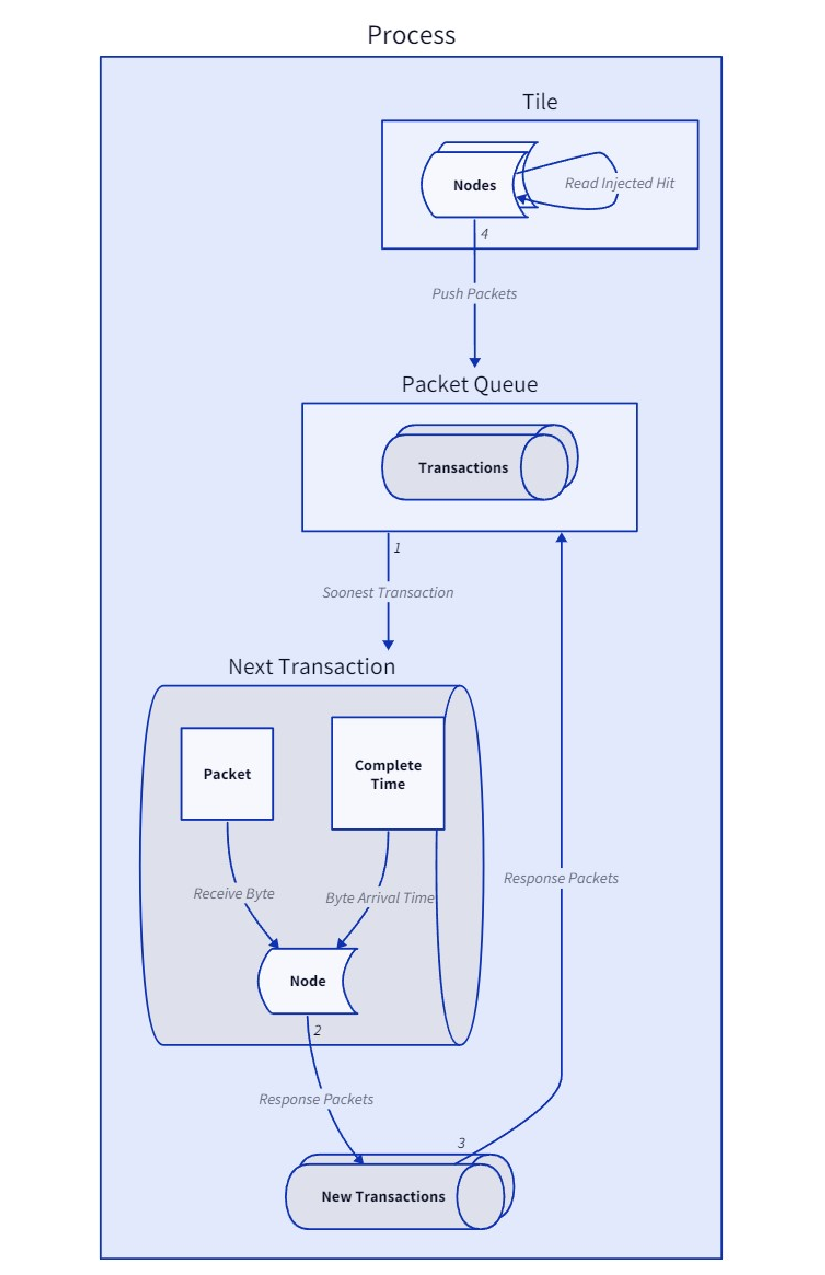
\includegraphics[width=0.65\textwidth]{images/simulation_process_method.pdf}
\caption{Flow chart of the simulation process method which occurs for every simulation time step.
The simulation contains a queue of packet transactions.
The queue is sorted by ascending time, so that the earliest transaction completed time is processed first.
Each transaction contains a packet, a node, and the time the packet arrives.
When the node receives the packet, it can optionally create more transactions, depending on the node's state and the packet.
Any additional transactions are added to the simulation queue, and are time sorted.
The simulation then increments the time for all other nodes within the tile.
This procedure repeats until all nodes in the tile reach the designated time (11~\unit{seconds}).
}
\end{figure}~\label{fig:simulation_process_procedure}

A transaction represents a 64-bit packet that is transferred between two nodes (Sect.~\ref{sec:comms}).
The sending node is responsible for calculating the true time when this transaction would complete.
The receiving node records this byte onto its remote FIFO and performs the state check based on this packet according to Fig~\ref{fig:digital_fsm}.
Then the receiving node updates its time to its soonest clock cycle after this transaction completed.
Next, each node in the entire tile is processed one forward timestep.
If nodes are in the push state and receive a hit within this timestep window, they create a new outgoing packet, and add this packet to the transaction queue.
We note that it is only possible for processed nodes which did not receive the transaction packet to create a new packet if they are in a push-based architecture. 

The simulation is complete when all nodes have been processed up to the final requested time and no transactions are left in the queue. 
In the results presented here we process the tile for one second longer than any injected resets to ensure that the tile is fully read out.


\section{The Tile Parameters}

One goal of the simulations presented here is to parameterize different design choices in constructing both the digital nodes and the tiles.
The different parameters which we test are described in Table~\ref{table:tile_params}.

There are a total of four parameters to test: frequency stability, tile size, routing, and architecture.
Of the four parameters, we note that the frequency stability is the one parameter determined by the ASIC's physical design.
Therefore, special care must be taken into account when designing the local oscillator for the ASIC.
The other variables: routing, architecture, and tile size are either programmable registers or easily configurable in hardware layout.

It is intuitive (and the results indicate) that improved frequency stability leads to a more stable design.
Nevertheless, we find it enlightening to demonstrate how remote buffer depths are affected in the case of a 5\% (0.5\%) clock deviation.
When a tile is created with 5\% (0.5\%) frequency deviation each node within the tile is created by randomly sampling from a Gaussian distribution with a mean of 30$\unit{MHz}$ and a standard deviation of 5\% (0.5\%).
Since many ($\approx 10^4$) events are performed per tile configuration each tile is created with a random seed to ensure that each node is created with the same frequency for each test.

\begin{table}
\begin{center}
\begin{tabular}{|| p{30mm} | p{30mm} | p{90mm} ||}
 \hline
 Parameter & Values Taken & Description \\ [0.5ex]
 \hline\hline
  Oscillator\newline Frequency & 0.5\%, 5\% & High variance causes packet buildup or drift within the tile depending on whether packets are sent from slow to fast, or fast to slow clocks. \\
 \hline
  Tile Size & 4$\times$4, 8$\times$8\newline 10$\times$14, 16$\times$16 & Affects total number of resets which must be routed to aggregator.\\
 \hline
  Routing & Snake, Left, and Trunk & Tiles with different routing are effectively different graphs which affect packet buildup~(\ref{eq:adjacency_matr}). Different combinations of edges between nodes can cause packet buildup if nodes have more input edges than output edges.  \\
 \hline
  Architecture & Push, Pull & Describes conditions for when node enters transmit-local state.~\ref{sec:local_data_packet}. The push architecture allows individual nodes to transmit data when data are received, whereas pull architecture only send data upon receiving a special request packet from the aggregator.  \\
 \hline
\end{tabular}
\caption{The different tile parameters that are used for the effective tile search.
  The frequency drift relates the relative distribution of the frequency of adjacent oscillators.
  The tile size determines how many digital nodes are within a single tile.
  The routing configurations are described in detail in the previous chapter, and refer to how local data words are sent to the aggregator.
  The two different architectures define how the node enters the transmit local state.
  The push architecture enters whenever a new reset is acquired, whereas the pull architecture enters only when a data request is received from the aggregator.}
\label{table:tile_params}
\end{center}
\end{table}

The other design parameters are readily configurable in either hardware (tile size) or through register configurations of the digital node (routing and, possibly, architecture).
Tile size is mostly an engineering and cost constraint.
Larger tile sizes mean the full design would require less aggregator nodes and require less tiles to parameterize.
We show results for small tile sizes to indicate possible connections portions of larger tiles could configure.
The largest tile size we tested was 16 $\times$ 16 as the current limit in the Q-Pix digital prototype only allocates four bits for each x or y coordinate in a tile.

The routing and architecture parameters help guide the digital design efforts design of the digital ASIC.
In practice it is all but certain that implemented routing for a digital tile will take on a combination of the routing styles described here.
The reason for this is simply that is likely that some digital nodes will fail (for whatever reason) in the life time of a DUNE-FD 10 kT module.
Therefore, future tiles that contain hybrid routing we suggest to those users to individually analyze the sub tiles with appropriating routing and frequency distribution and determine if the buffer depths are appropriate.

\subsection{Oscillator Frequency and Drift}

Two different oscillator frequencies are tested, as shown in Table~\ref{table:tile_params}.
These different frequency variances indicate mean differences in oscillator frequency between adjacent nodes.
An example of the 5\% oscillator variance is shown in Figure~\ref{fig:asic_frequency_example}.
The values plotted in this figure indicate relative factors above or below the expected 30\unit{MHz} mean.

Local oscillator drift was not included as a testing parameter since transactions occur over small time scales compared to any likely meaningful oscillator drift.
If these drifts occur on time scales much longer than the interrogation time than the oscillator, the frequency could be continually re-calculated with the method shown in the previous chapter.
If these drifts are periodic about a mean frequency and on time scales much smaller than the interrogation time window then the drifts would average out.
In the event that clock drift timescales are on the interrogation timescale ($\approx 1\unit{s}$), then this is equivalent to a frequency uncertainty for the entire transaction cycle.
This would mean that an oscillator has a $\approx 5\%$ uncertainty in its frequency on each interrogation.
Such a node would not be able to reconstruct timestamps, and therefore not be able to reconstruct the z-position of charge with the required 1$\unit{ppm}$ estimated uncertainty for Q-Pix clocks~\citep{qpix:nygren:mei}.

\begin{figure}[]
\centering
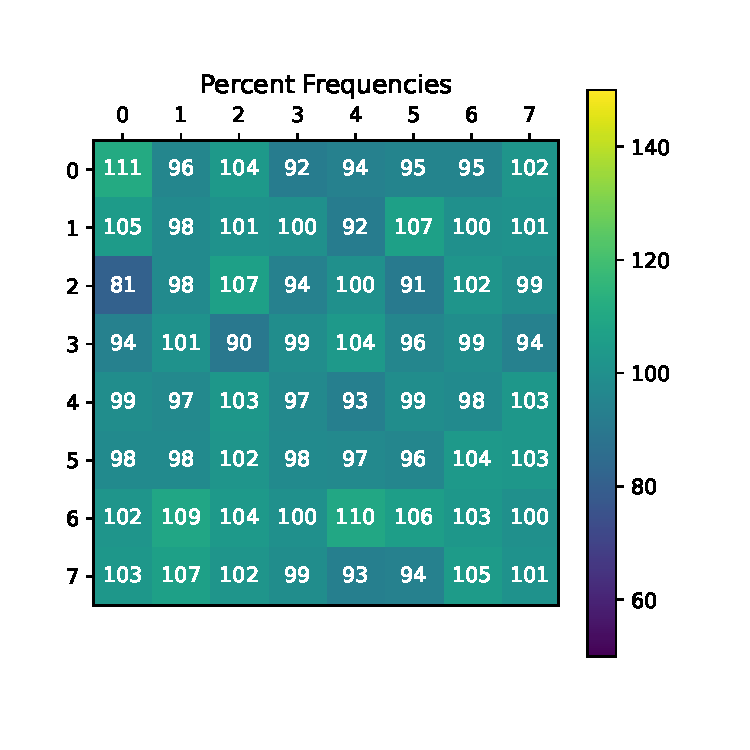
\includegraphics[width=\textwidth]{images/asic_frequency.pdf}
\caption{Distribution of ASIC frequencies used in the 8$\times$8 tile, and in the example FIFO buffer depths for this chapter.
The numbers plotted above each ASIC row and column indicate the relative frequency of this ASIC compared to the nominal 30$\unit{MHz}$ mean.
For example, a number of 112 indicates an ASIC which is 12\% faster than 30MHz, a frequency of $\approx 33.6 MHz$.}
\end{figure}~\label{fig:asic_frequency_example}

\section{Simulating The Tile Readout}~\label{sec:simulating_tile}

The tile simulation is performed by injecting hits from two known sources: radiogenic backgrounds and beam neutrinos.
All results presented in this chapter are based on 11 seconds of simulated run time.
Radiogenic data are collected and used to occupy 10 seconds of background noise resets.
The higher intensity neutrino events are offset so that interaction occurs at $t = 5.1 s$.
The simulation is run for a total of 11 seconds, instead of 10, to ensure that all of the packets are collected by the aggregator node.
In practice, there would be additional resets from backgrounds which occur in that final second of data.
However, the number of resets from the radiogenic events are much smaller (by about two orders of magnitude) than the neutrino events.

The full readout of the tile occurs based on the number of packets times the average transaction length.
\begin{equation}
T_{\mathrm{readout}} \approx 50 \mu s \times N_{\mathrm{max}}
\end{equation}

If we set $T_{\mathrm{readout}}$ to 1 second:
\begin{equation}
N_{\mathrm{max}} \approx 20000
\end{equation}

Since the simulation is run six seconds longer than the origin time of the neutrino events all reset events are be accounted for if neutrino events cause less than $\approx 120000$ resets.
There are no simulated neutrino events which create these number of resets since this would require an energy of $\approx$ 15\unit{GeV} deposited into the LAr.

The configuration of each node and the tile happens before the beginning of the simulation.
The frequency and the routing directions are configured for each node during its creation.

\subsection{Simulation Timing}

The purpose of the simulation is the examine the communication behavior of digital nodes at different frequencies which communicate via packets of variable time width.
For this reason special care is taken to ensure that the timing of packet transactions in the simulation are accurate.
The behavior of each node is determined by its state machine properties, as described in Fig.~\ref{fig:digital_fsm}.
Therefore, an accurate measure of timing for each node is equivalent to ensuring that timing of ASIC state transitions are accurate.

%% example snake route
\begin{figure}[]
\centering
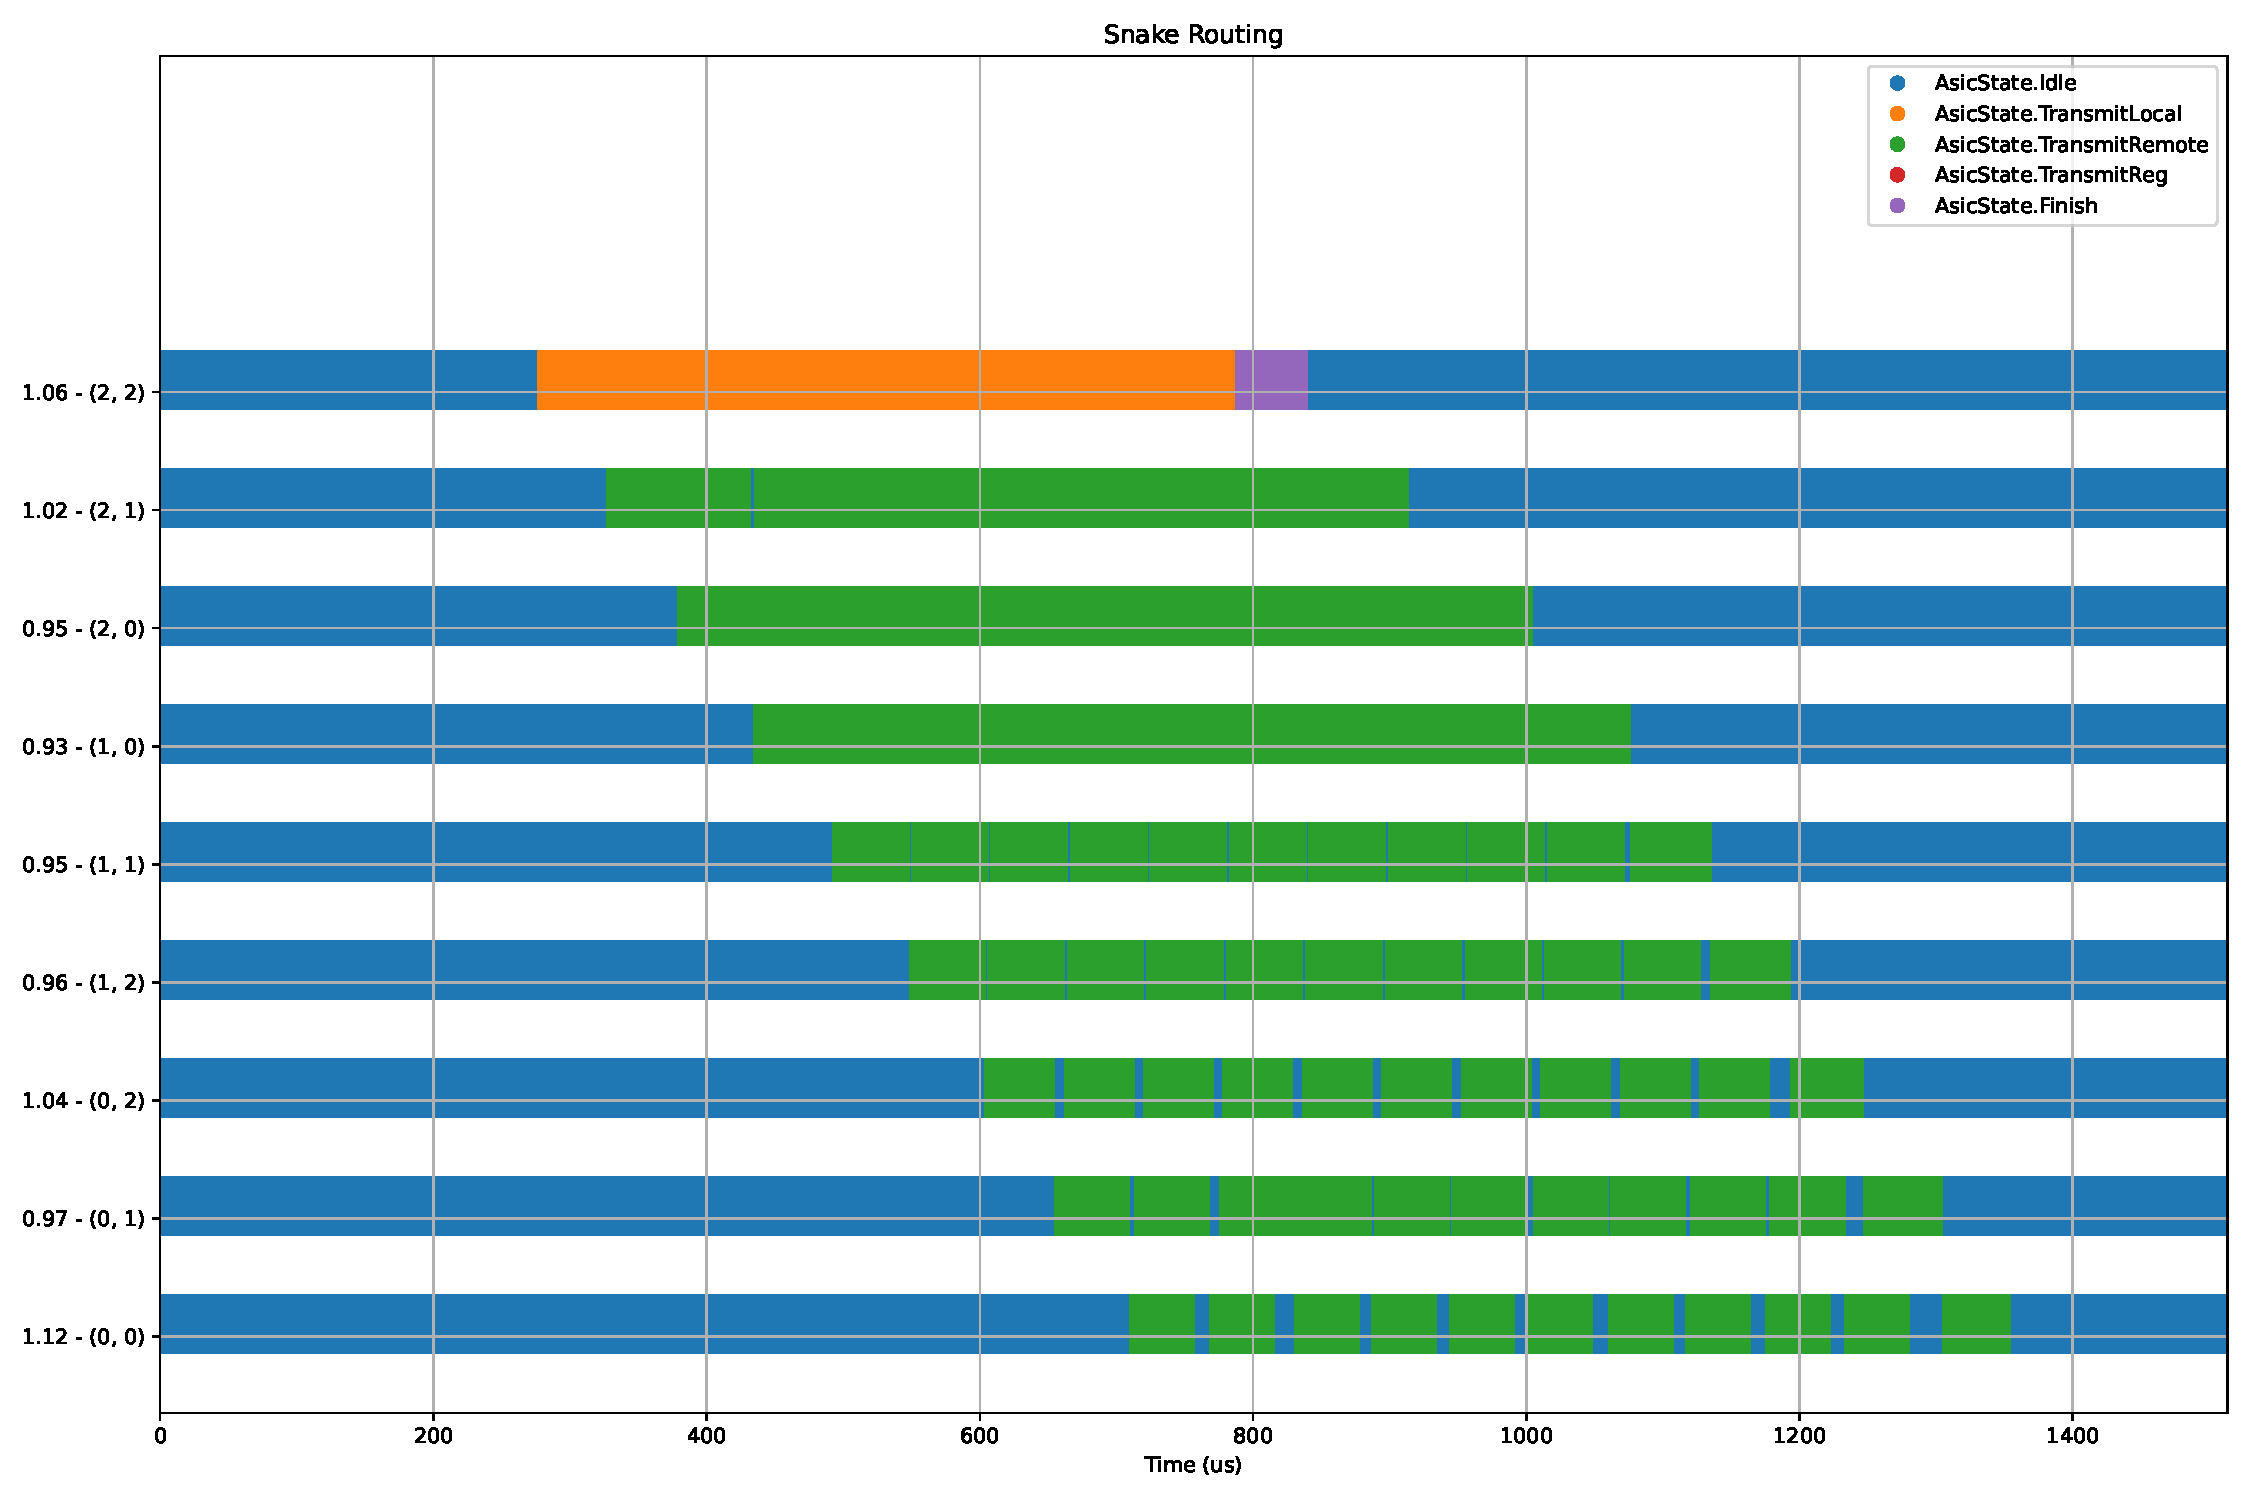
\includegraphics[width=\textwidth]{images/snake_timer.pdf}
\caption{Example of timing ASIC state transitions in the simulation framework.
  The x-axis represents time in $\mu s$, and the different y-axis labels represent different ASICs within a 3$\times$3 tile shown.
  The y-axis also indicates the relative frequencies of the ASICs in the tile, where the node at (0,0) has the fastest frequency, which is 12\% faster than 30 MHz.
  The blue regions indicate that the ASIC is in the idle state.
  The first orange state indicates that this ASIC (2,2) received a register request from the aggregator node and is now sending its local data, concluding in the purple state, which is sending the event end word.
  The Packets drift apart in time as they are sent from slower to faster ASICs.
  Shown here is the possibility of packet drift due to asynchronous packet transfers that depends on the magnitude of the frequency drift between neighbor ASICs.
}
\end{figure}~\label{fig:snake_packet_drift}

Not shown are times when an ASIC receives or responds to a broadcast.
Broadcast packets are uniquely handled by ASICs.
An ASIC, instead of writing the request to the remote FIFO, immediately handles a broadcast by sending this packet to all neighbor ASICs, excluding the direction from which it received the broadcast.
This means that an ASIC's state does not change during a broadcast.
This is handled by the simulation by tracking packet times on the ASIC connections.
The broadcast packet is sent starting at the soonest available time on each connection.
The full broadcast procedure is described in Section~\ref{sec:broadcast}.


\subsubsection{Snake Timing Example}~\label{sec:snake_timing}

Here we refer to the "snake" routing as the maximal path routing.
This routing is one that minimizes the number of input edges for all nodes within a tile.
An example of a packet transfer which uses this routing is shown in Figure~\ref{fig:snake_packet_drift}.

Since the snake routing minimizes the number of edges, it also maximizes the number of ASICs responsible for sending remote data in the tile.
This increases the number of remote transactions in a tile readout.
This demonstrated by the amount of time ASICs are in the transmit remote state shown in Figure~\ref{fig:snake_packet_drift}.

%% example local vs remote of snake
\begin{figure}
\centering
\begin{subfigure}{.5\textwidth}
  \centering
  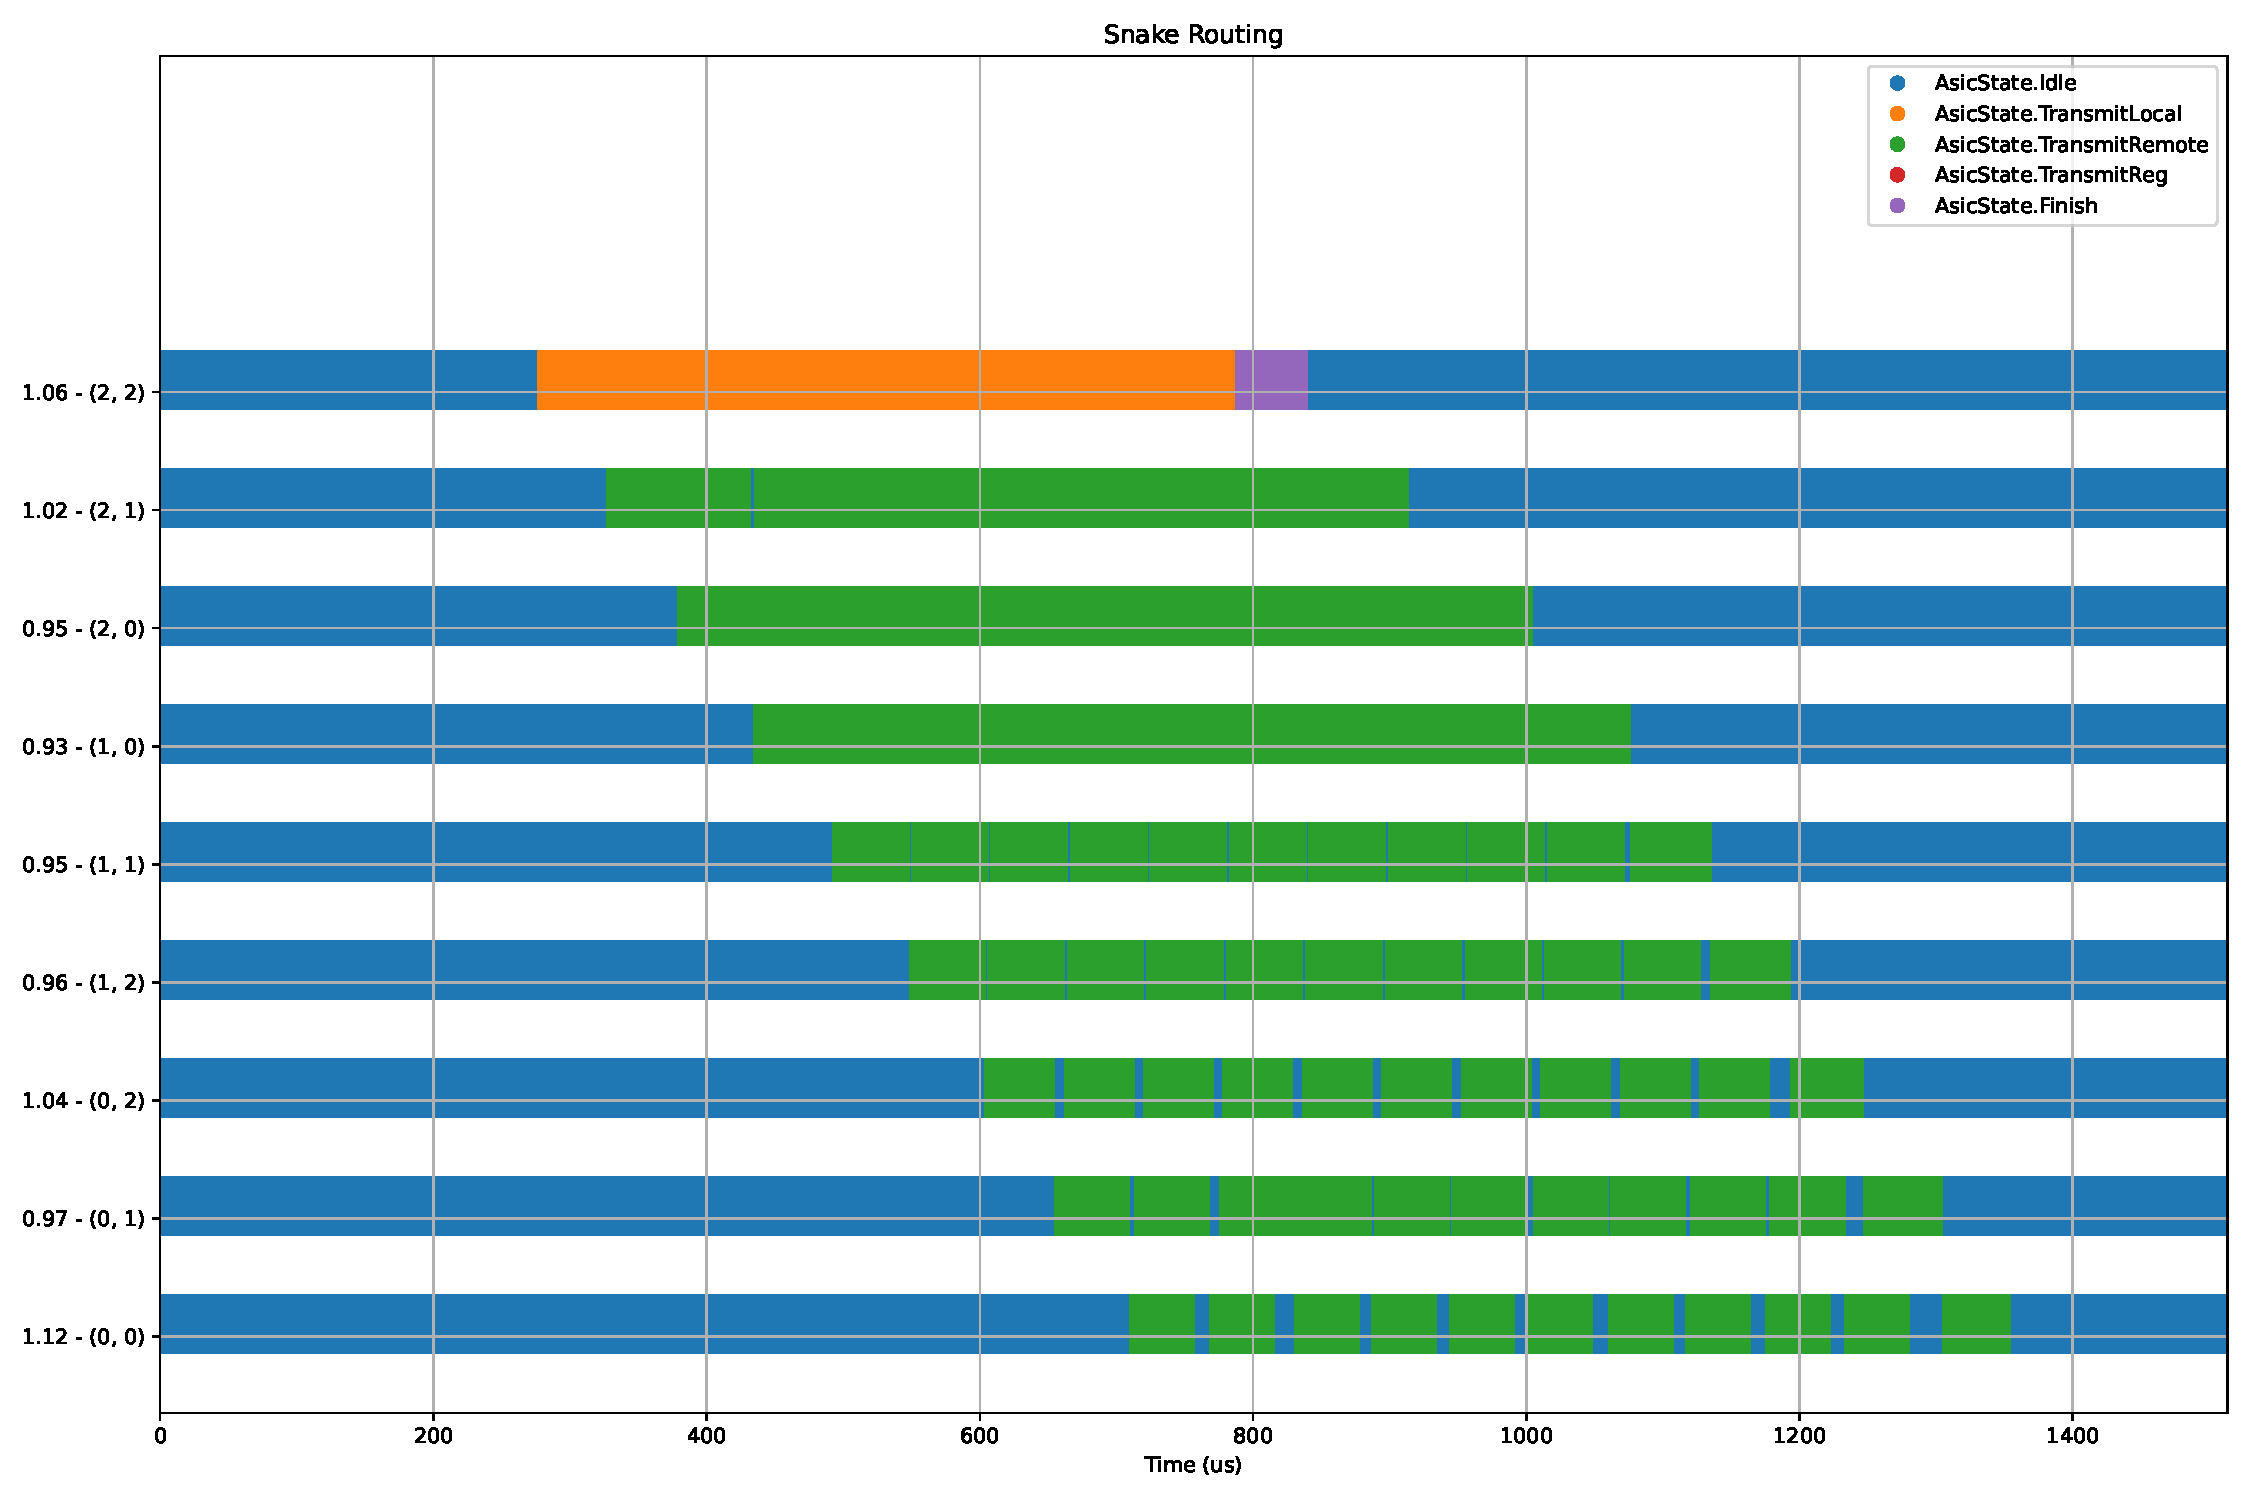
\includegraphics[width=\textwidth]{images/snake_timer.pdf}
  \caption{Snake Readout timing Diagram}
\end{subfigure}%
\begin{subfigure}{.5\textwidth}
  \centering
  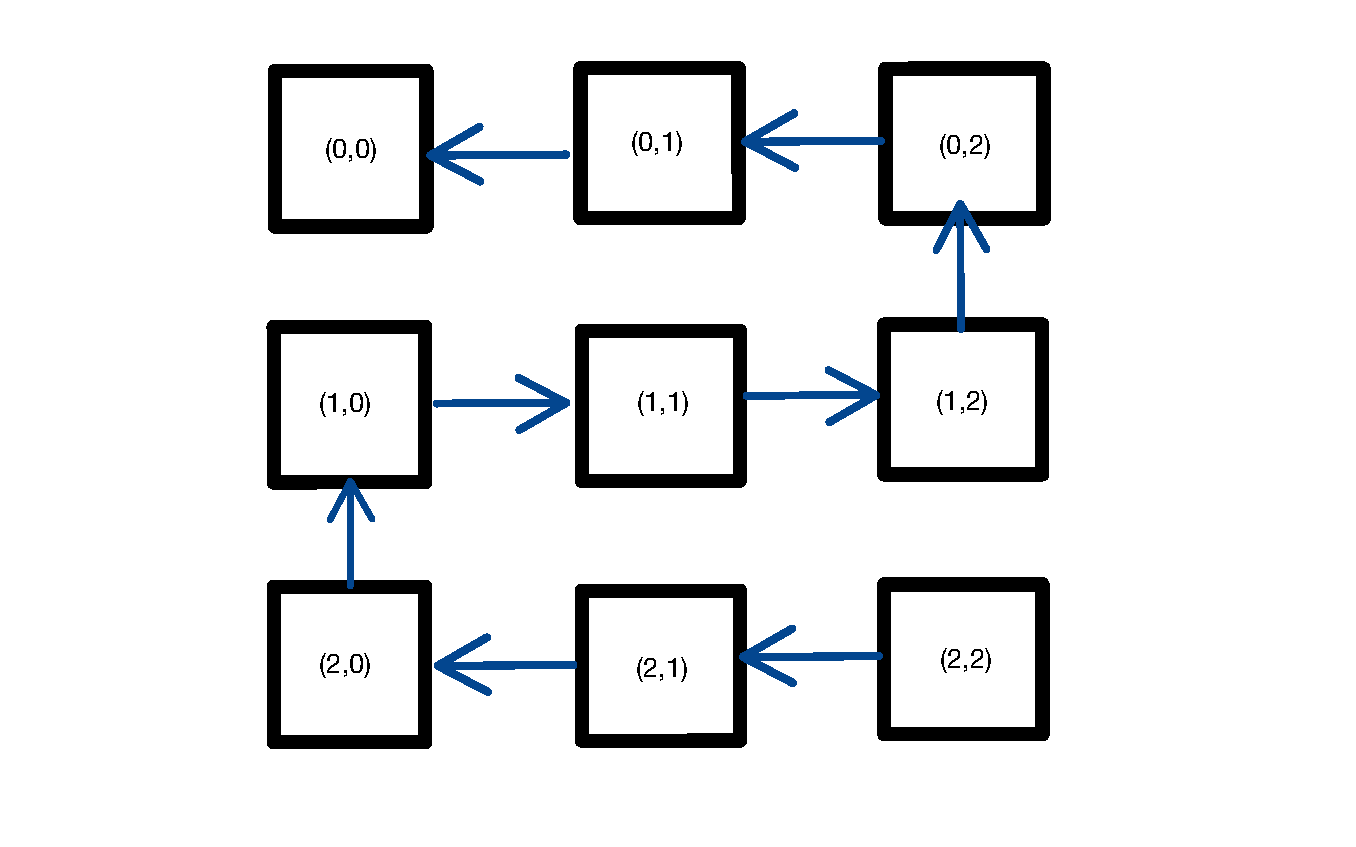
\includegraphics[width=\textwidth]{images/snake_ex_read.pdf}
  \caption{Data Path in Snake Readout}
\end{subfigure}
\caption{A snake packet transaction example is shown. The broadcast is received by the further node (2,2) and 10 data words are sent, followed by a event end word.
Each packet traverses through all nodes in the tile where remote packets are sent immediately.}
\label{fig:snake_timer}
\end{figure}

%% example left route
\subsubsection{Left Timing Example}

The naming convention for the "left" routing is arbitrary since the tile can be viewed from the opposite direction and the routing would appear "right".
By "left" routing we mean a routing configuration in which the routed direction for all ASICs in all rows are in the same direction, except for the nodes which have no neighbor in that direction.
These nodes then are routed "up" towards the aggregator.
An example of a packet transfer with this routing configuration is shown in Figure~\ref{fig:left_packet_drift}.

This routing configuration minimizes the path length for all nodes in the tile when the base-node is at the corner.

\begin{figure}
\centering
\begin{subfigure}{.5\textwidth}
  \centering
  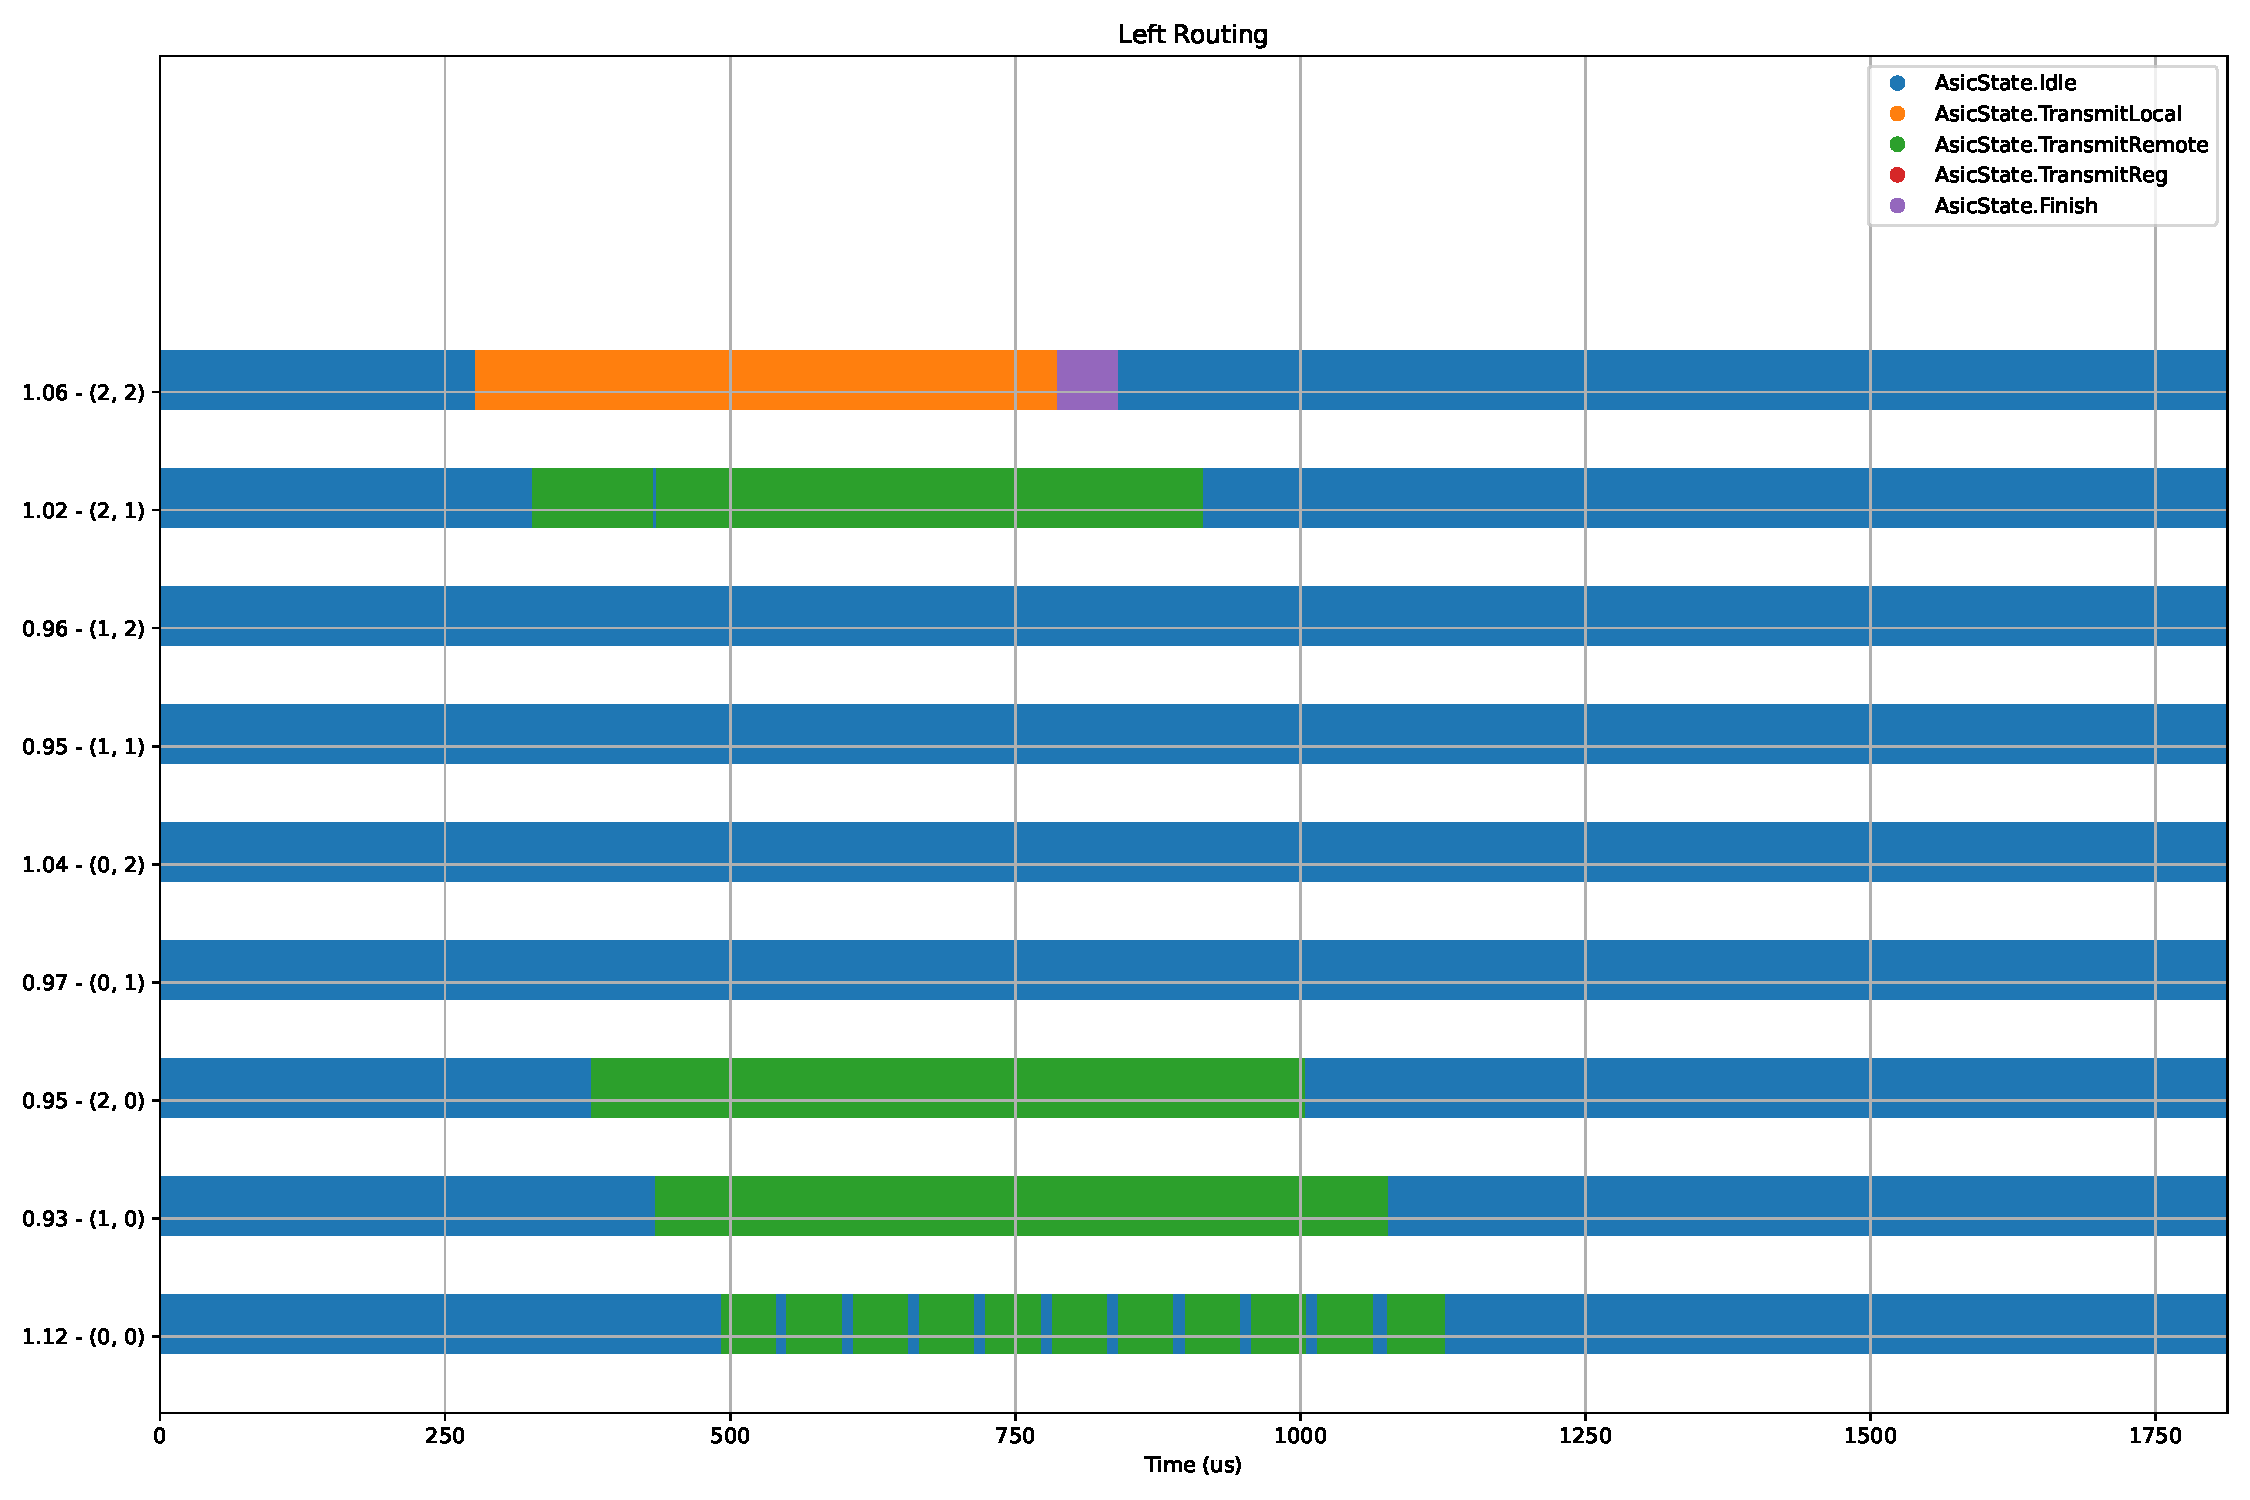
\includegraphics[width=\textwidth]{images/left_timer.pdf}
  \caption{Left Readout timing Diagram}
\end{subfigure}%
\begin{subfigure}{.5\textwidth}
  \centering
  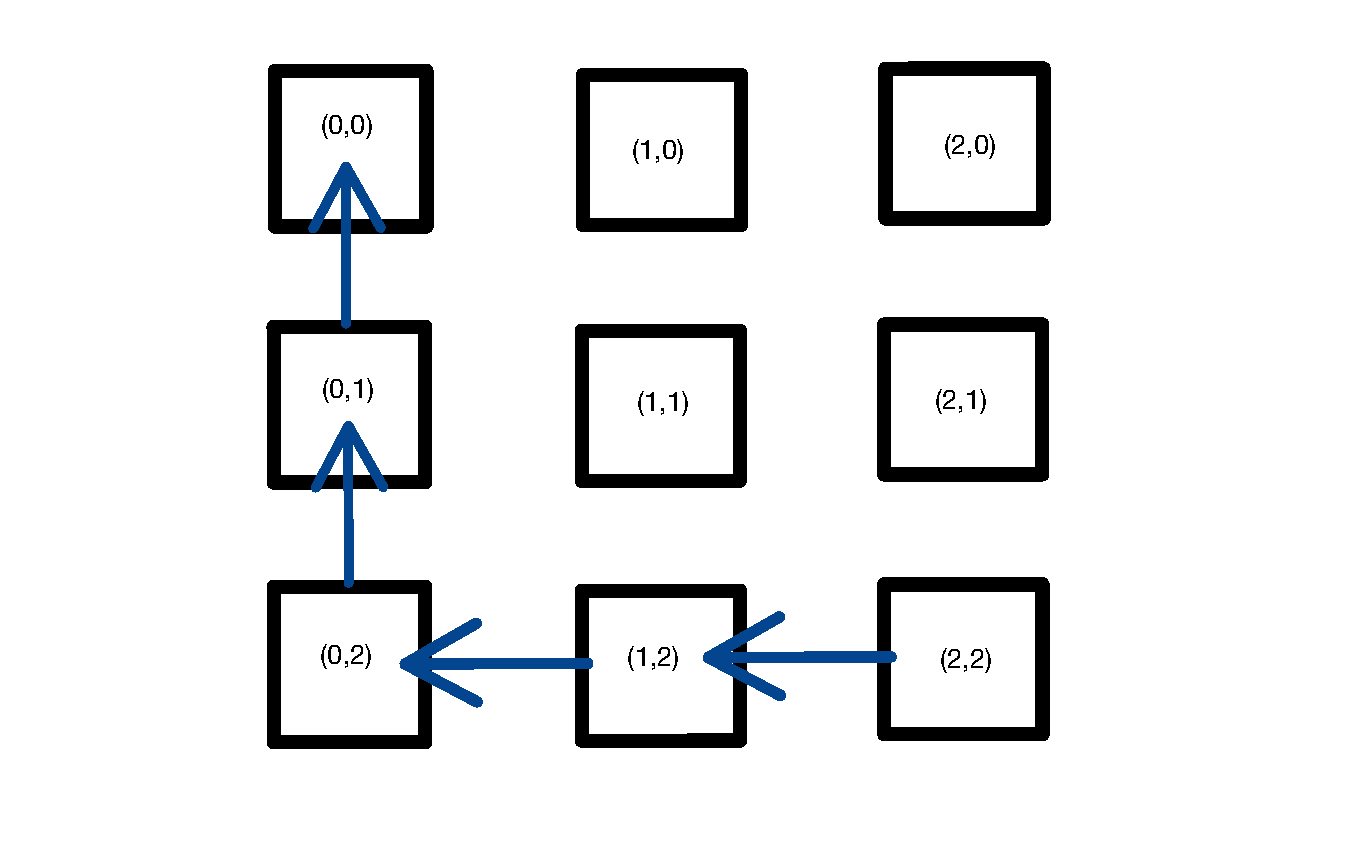
\includegraphics[width=\textwidth]{images/left_ex_read.pdf}
  \caption{Data Path in Left Readout}
\end{subfigure}
\caption{A left packet transaction example is shown. The packet transfers begin with the furthest node (2,2) receives a broadcast from the aggregator. 
The data are then sent to the "left" and then "up" towards the base node, and finally to the aggregator node.}
\label{fig:left_packet_drift}
\end{figure}


\subsubsection{Trunk Timing Example}

The final routing scheme we simulate we call the "trunk" routing.
We name this routing the "trunk" because all data are sent to a central column within the tile and then up towards the edge base node.
An example of a simple data transfer is shown in Figure~\ref{fig:trunk_packet_drift}.

For tiles of widths larger than three there are multiple choices for which column will be the trunk.
In for example, a 4$\times$4 tile can have either the second or third columns be the trunk.
In all even width cases we test, we choose the smaller row value for simplicity.
In the 4$\times$4 case we choose the second column and in the 8$\times$8 case, we choose the fourth (3,0) column instead of the fifth (4,0).

\begin{figure}
\centering
\begin{subfigure}{.5\textwidth}
  \centering
  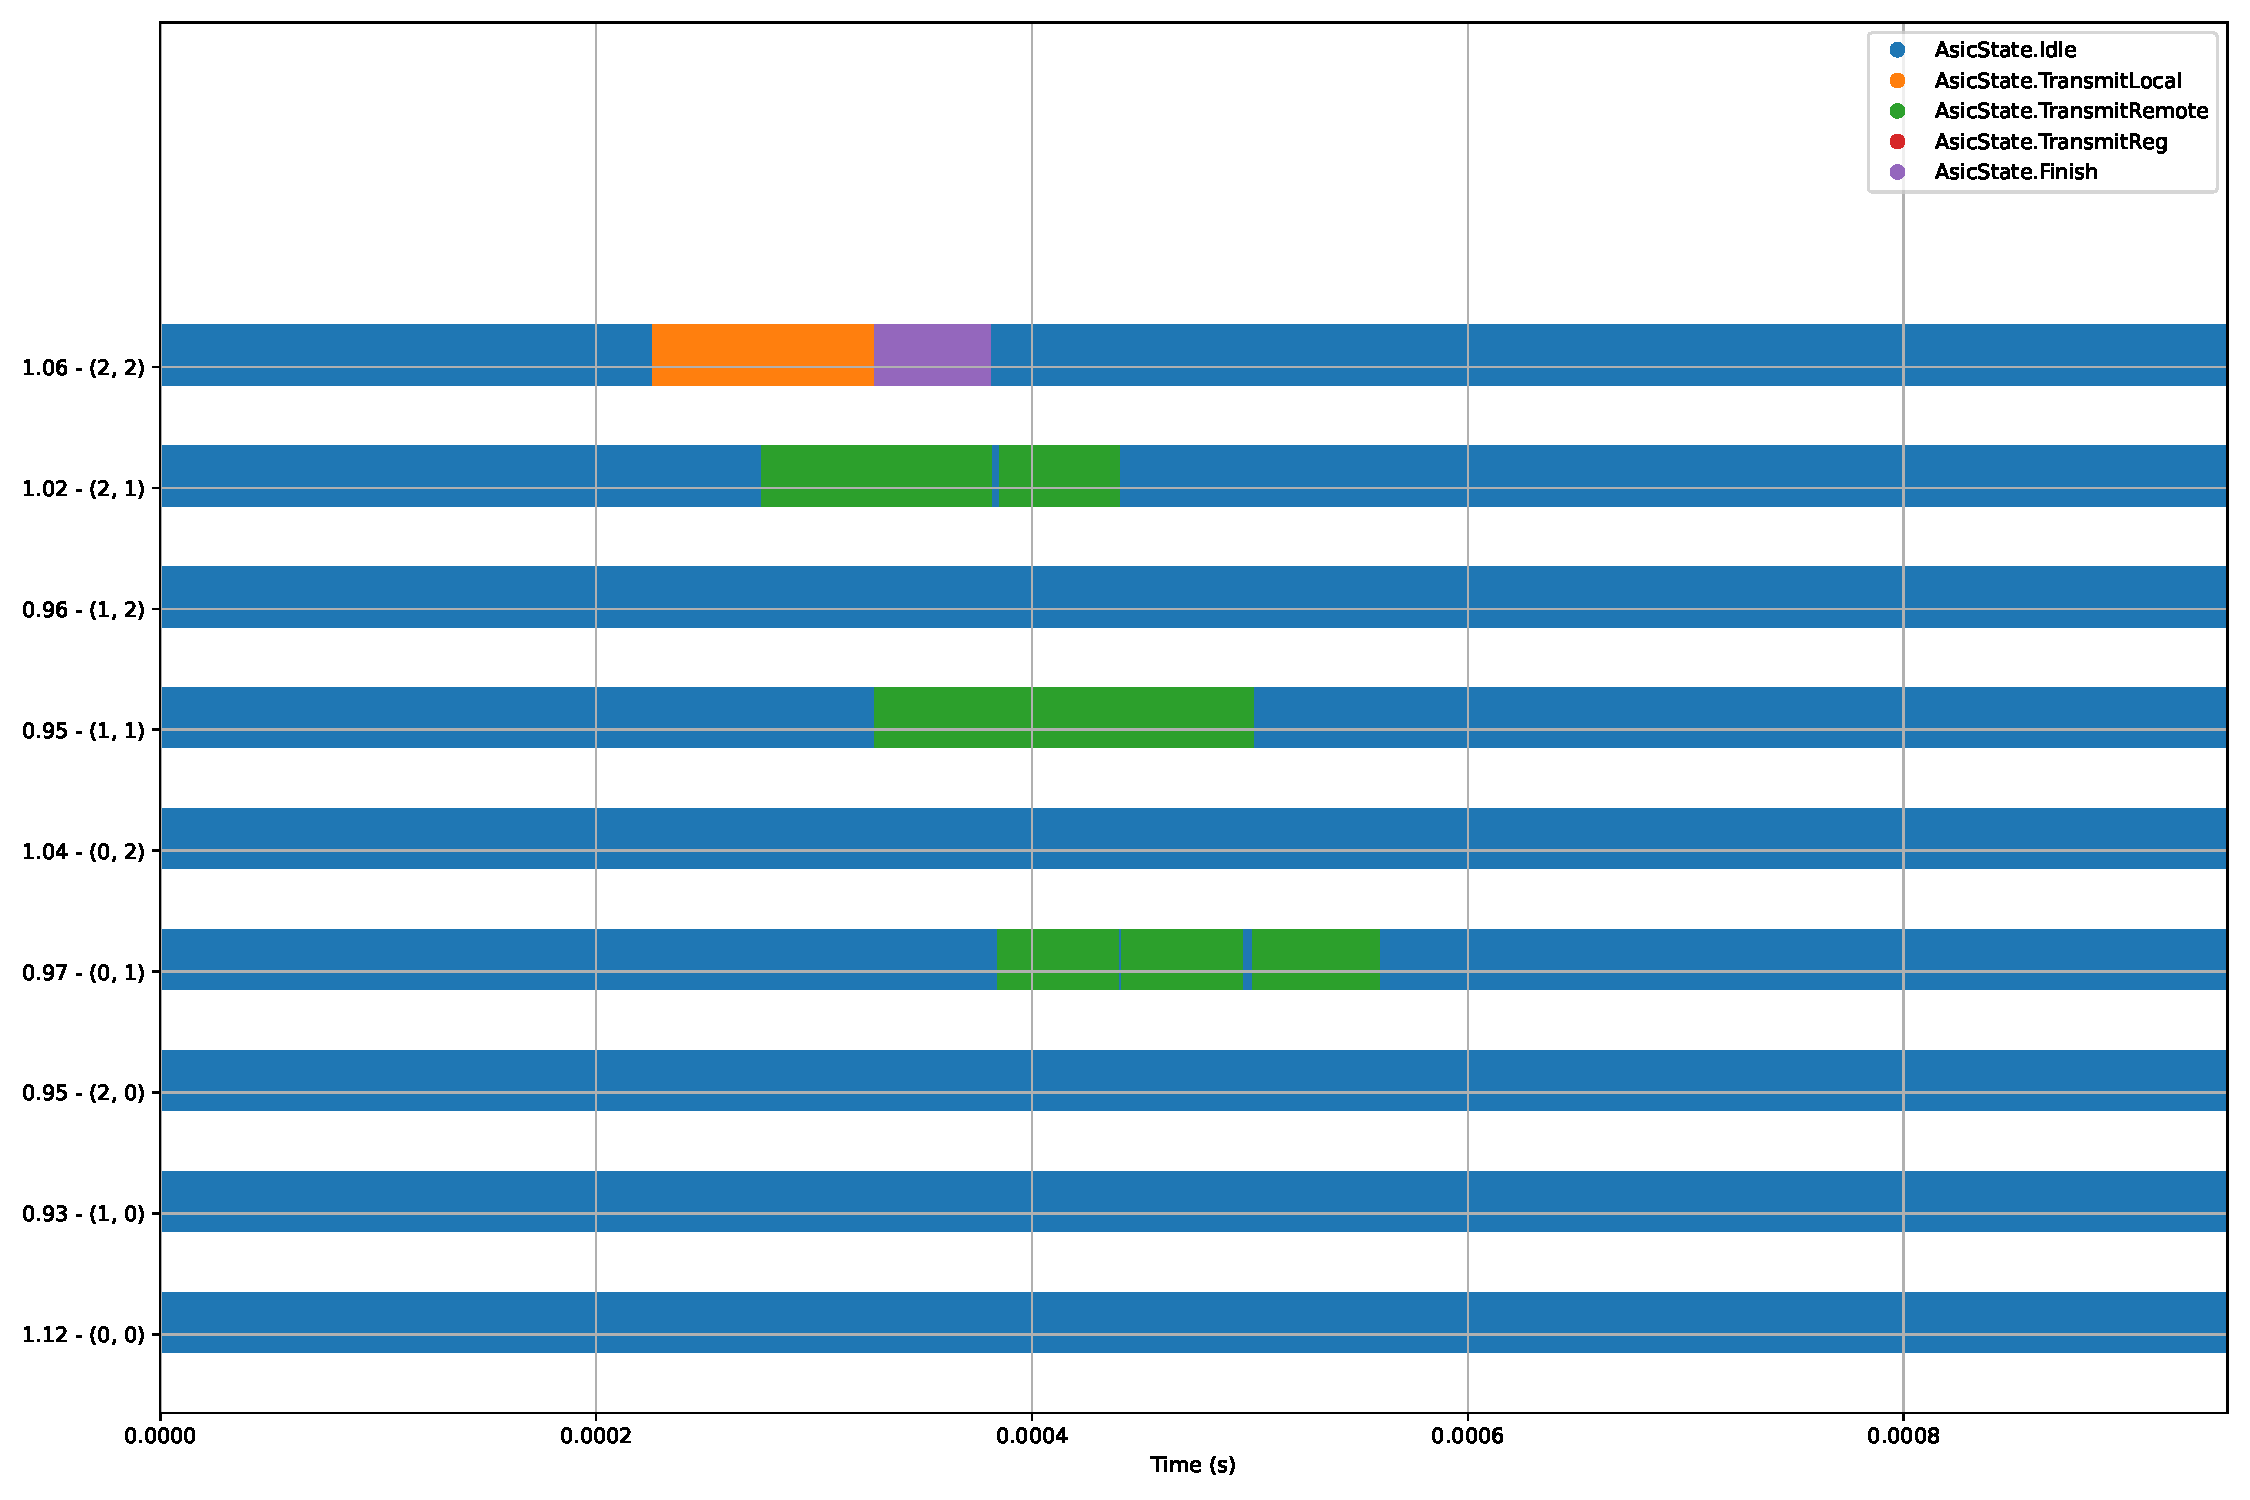
\includegraphics[width=\textwidth]{images/trunk_timer.pdf}
  \caption{Trunk Readout timing Diagram}
\end{subfigure}%
\begin{subfigure}{.5\textwidth}
  \centering
  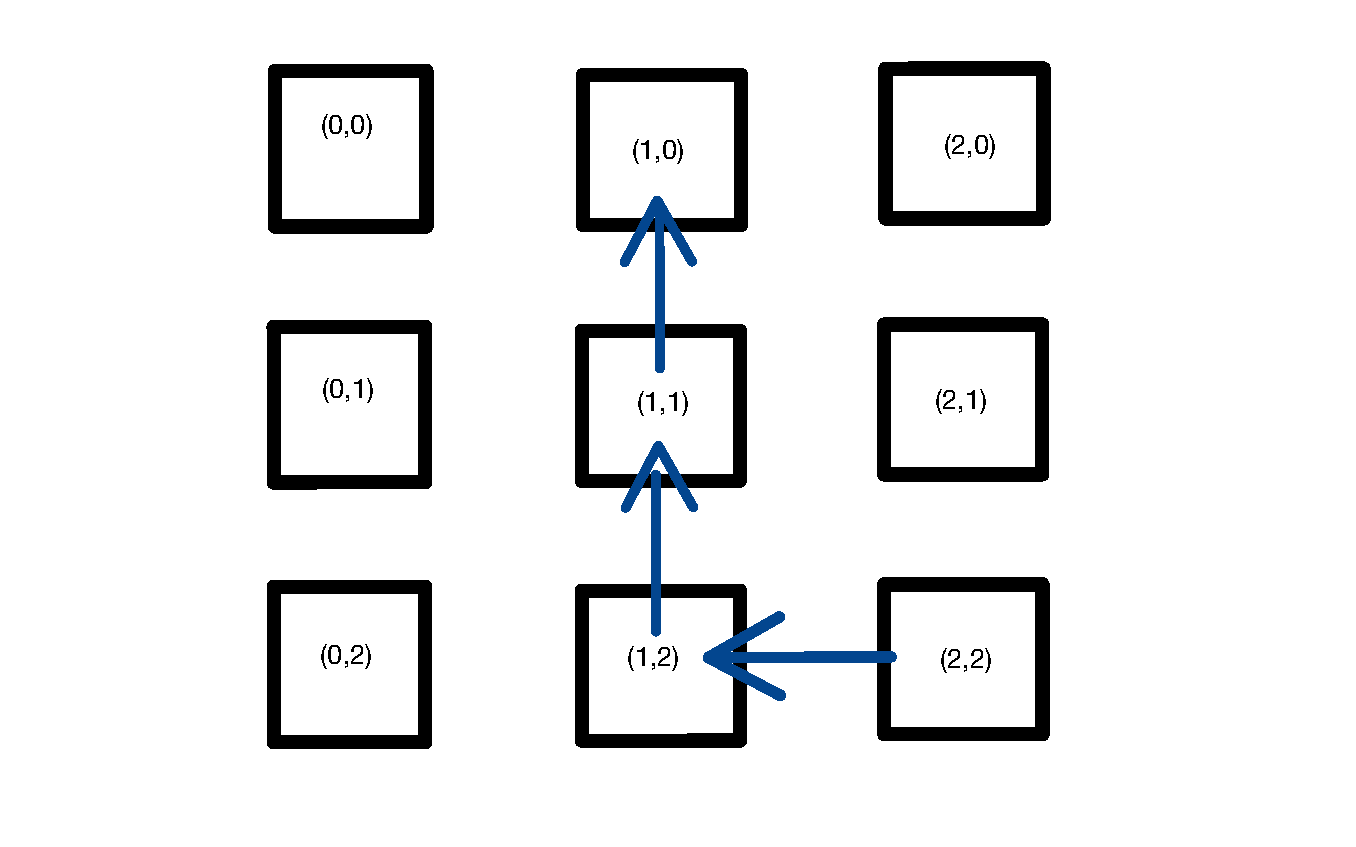
\includegraphics[width=\textwidth]{images/trunk_ex_read.pdf}
  \caption{Data Path in Trunk Readout}
\end{subfigure}
\caption{A trunk packet transaction example of two data words and a single event end word is shown. 
This routing method allows for the fastest possible transaction time since it minimizes the edge lengths between the base node and all other nodes within the tile.
In this 3$\times$3 example shown, the base node is at (1,0), or in the middle.}
\label{fig:trunk_packet_drift}
\end{figure}


\subsection{The Pull Architecture and FIFO Depths}

The "pull" architecture describes a tile configuration where data are only sent by ASICs within the tile when they receive a broadcast packet.
We describe an example simulation event in this section with the pull architecture and the three routing methods to demonstrate which variables are recorded.
The example presented in Figure~\ref{fig:local_buffer_hit_example} stores resets accumulated over ten seconds from both radiogenic backgrounds and a 3$\unit{GeV}~\nu_{e}$ event.
The data shown are the total local FIFO transactions (writes) that occurred in the ten second run.

The figures shown in~\cref{fig:snake_example_neutrino,fig:left_example_neutrino,fig:trunk_example_neutrino} demonstrate how the data are accumulated onto the remote FIFO depths for the snake, left, and trunk routings respectively.

%% example local hits
\begin{figure}[]
\centering
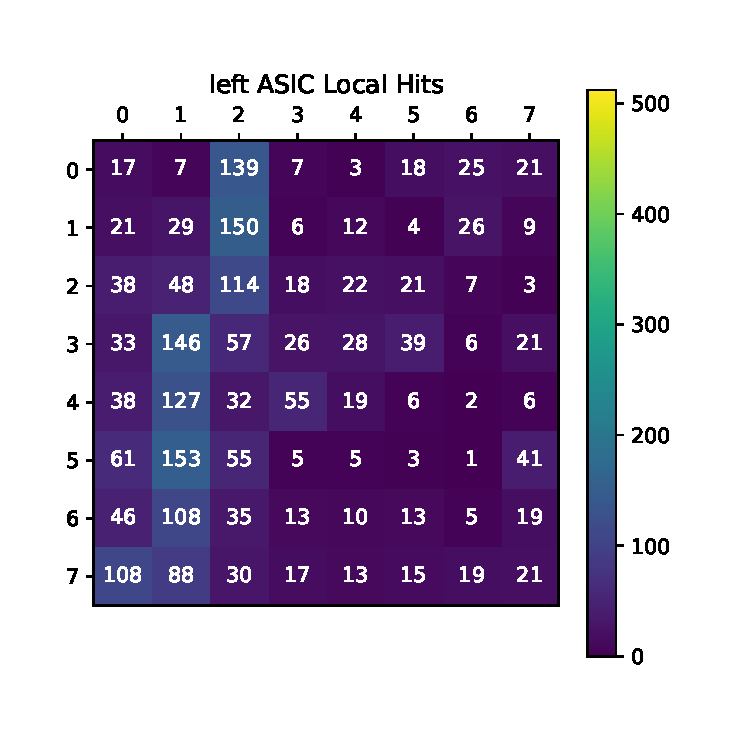
\includegraphics[width=0.75\textwidth]{images/left_asic_local.pdf}
\caption{Example local FIFO distribution of a $\approx 3\unit{GeV}~\nu_{e}$ event.
The numbers over each tile represent the total number of writes which occurred to each local FIFO in the array.
Even with the lowered resolution (each ASIC accounts for 16 pixels), different tracks are noticeable based on the FIFO depths.
The maximum scale for the heatmap is chosen to be 512 resets.
}
\end{figure}~\label{fig:local_buffer_hit_example}


%% example local vs remote of sneak
\begin{figure}
\centering
\begin{subfigure}{.5\textwidth}
  \centering
  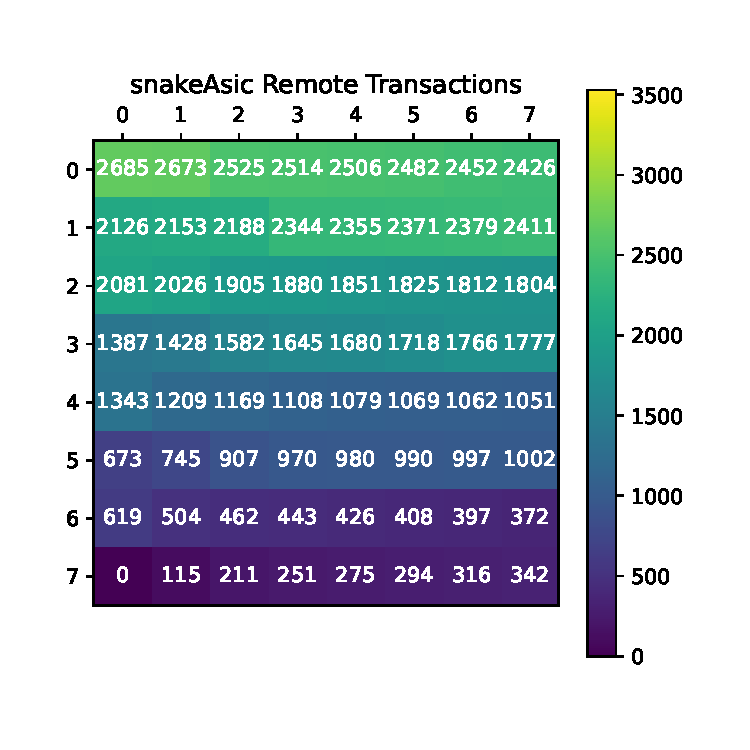
\includegraphics[width=\textwidth]{images/snake_asic_trans.pdf}
  \caption{Local FIFO Depths}
\end{subfigure}%
\begin{subfigure}{.5\textwidth}
  \centering
  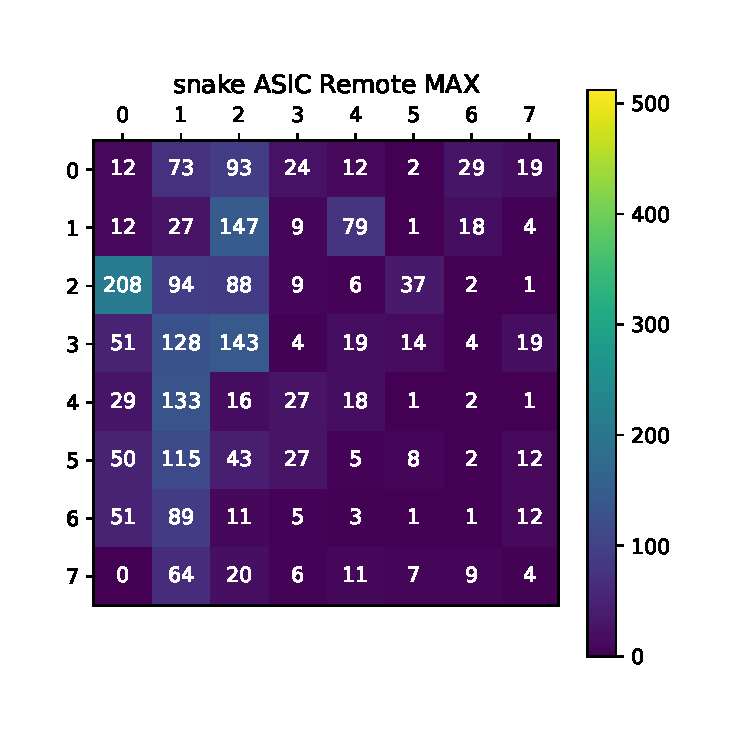
\includegraphics[width=\textwidth]{images/snake_asic_remote.pdf}
  \caption{Remote FIFO Depths}
\end{subfigure}
\caption{Example of local (a) and Remote (b) fifo depths of the example neutrino event from~\ref{fig:local_buffer_hit_example} after processing. 
The color bar to highlight the maximum number of transactions is used to indicate remote transactions which were happening for 2\% of the total readout time of 10 seconds.
The node which has the largest remote buffer depth corresponds to the ASIC with the slowest frequency as shown in Figure~\ref{fig:asic_frequency_example}.
The reason for this excess of buffer depth is due to packet buildup on the slow ASIC.
}
\label{fig:snake_example_neutrino}
\end{figure}


%% example local vs remote of left
\begin{figure}
\centering
\begin{subfigure}{.5\textwidth}
  \centering
  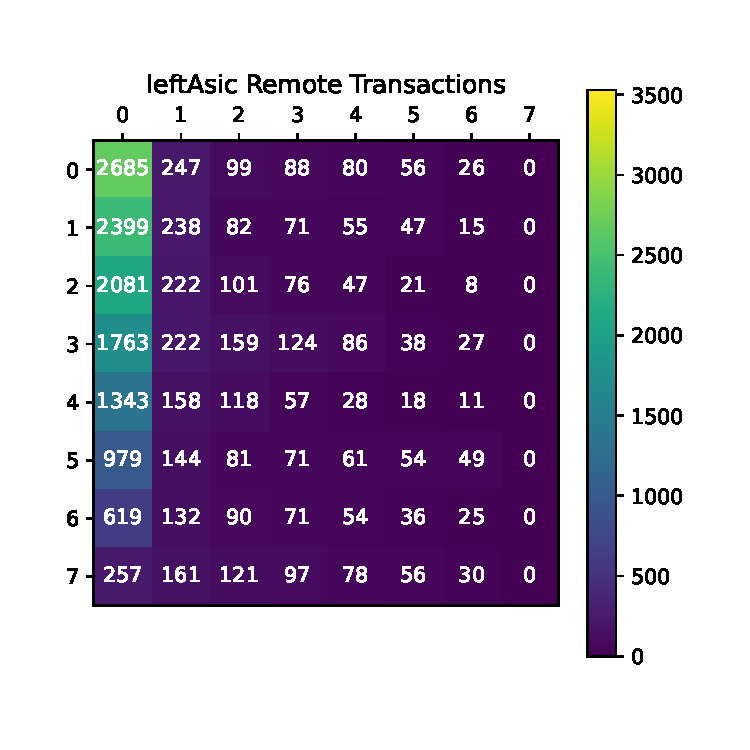
\includegraphics[width=\textwidth]{images/left_asic_trans.pdf}
  \caption{Local FIFO Depths}
\end{subfigure}%
\begin{subfigure}{.5\textwidth}
  \centering
  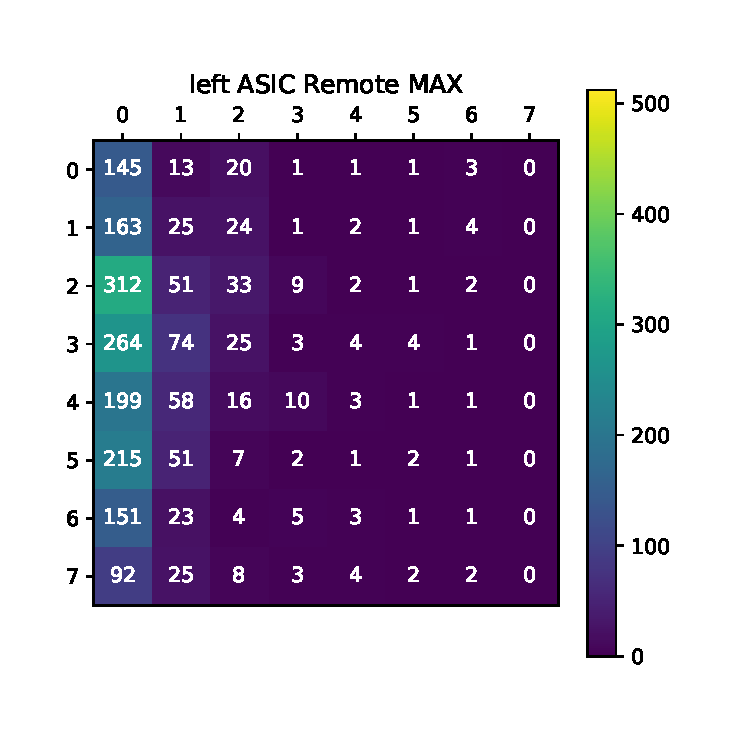
\includegraphics[width=\textwidth]{images/left_asic_remote.pdf}
  \caption{Remote FIFO Depths}
\end{subfigure}
\caption{Example of local (a) and Remote (b) fifo depths of the example neutrino event from~\ref{fig:local_buffer_hit_example} after processing.
 The ASIC which has the largest remote buffer depth also corresponds to the ASIC with the lowest frequency as shown in Figure~\ref{fig:asic_frequency_example}.}
\label{fig:left_example_neutrino}
\end{figure}

%% example local vs remote of trunk
\begin{figure}
\centering
\begin{subfigure}{.5\textwidth}
  \centering
  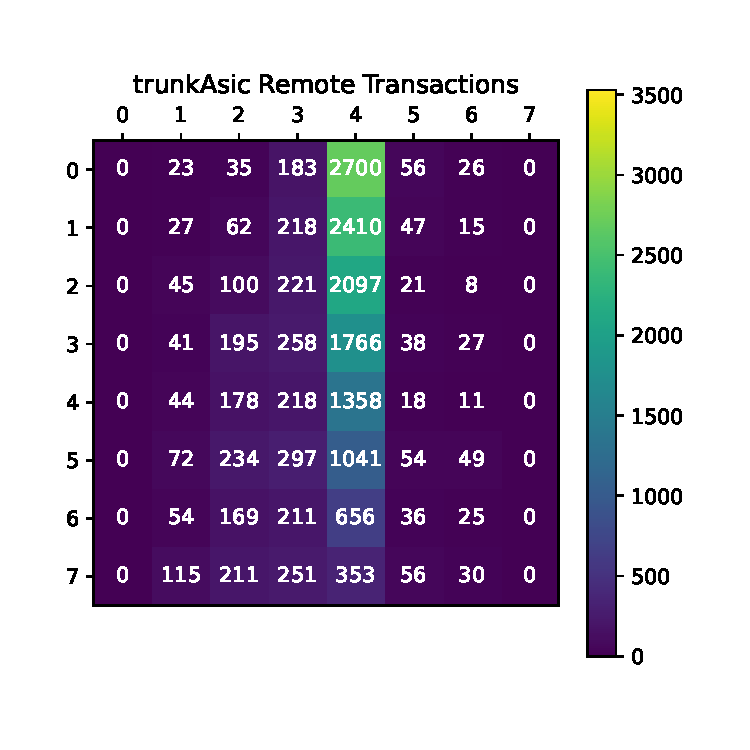
\includegraphics[width=\textwidth]{images/trunk_asic_trans.pdf}
  \caption{Local FIFO Depths}
\end{subfigure}%
\begin{subfigure}{.5\textwidth}
  \centering
  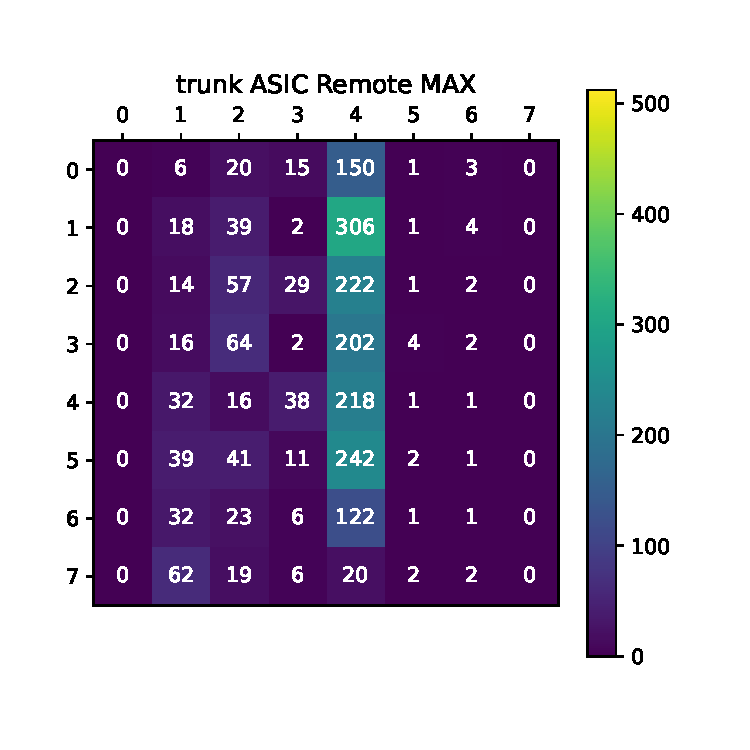
\includegraphics[width=\textwidth]{images/trunk_asic_remote.pdf}
  \caption{Remote FIFO Depths}
\end{subfigure}
\caption{Example of local (a) and Remote (b) fifo depths of the example neutrino event from~\ref{fig:local_buffer_hit_example} after processing.
The ASIC which has the largest packet buildup occurs at (4,1).
This ASIC also corresponds to the ASIC which has the lowest frequency along the trunk column as shown in Figure~\ref{fig:asic_frequency_example}.
}
\label{fig:trunk_example_neutrino}
\end{figure}


\begin{table}
\begin{center}
\begin{tabular}{|| p{20mm} | p{40mm} | p{40mm} | p{45mm} ||}
 \hline
 Routing & Local Max & Remote Maximum & Ratio of Remote:Local \\ [0.5ex]
 \hline\hline
  Snake & 153 & 208 & 1.36 \\
 \hline
  Left & 153 & 312 & 2.04 \\
 \hline
  Trunk & 153 & 306 & 2.00 \\
 \hline
 \hline
\end{tabular}
\caption{Example results obtained from the three simulation examples for the pull architectures shown in the previous figures.
The value of interest in determining the required remote FIFO depths for each ASIC is the maximum depth that occurred on any node.
A memory optimized routing configuration is one that would introduce the least strain on the remote buffer depths for a given local buffer depth input.
}
\label{table:example_analysis}
\end{center}
\end{table}

The following figures demonstrate why it is important to design all ASICs within a tile to meet the same specifications.
Future Q-Pix ASICs within a tile will be exposed to events at or above these energy scales, and there is no guarantee (until the ASIC is in hand) what the frequency of its oscillator will be, or its location within a tile. 
In all three routing examples shown it was not the base node which experienced the most strain on its buffer depth, but the ASIC along the route path which had the lowest frequency.


\subsection{The Push Architecture}

The final simulated parameter to describe is the push architecture.
Since the push architecture allows individual nodes to determine when packets can be sent all nodes must be inspected at each time step to check if a reset occurs before this new time window.
If a reset occurs at a time before the next simulation timestep, then the reset is removed from this node's hit list and is written to the node's local FIFO.
The node will then see at this simulation timestep that the local FIFO is not empty, and leave its idle state to send this packet.
An example of this process is shown in Figure~\ref{fig:push_arch_verification}.

Every simulated time step is shown and recorded along the x-axis.
The distance in time between simulation steps increases during packet transfers since the nodes state is fully determined during this time.
This simplification is performed to speed up simulation run time.

\begin{figure}[]
\centering
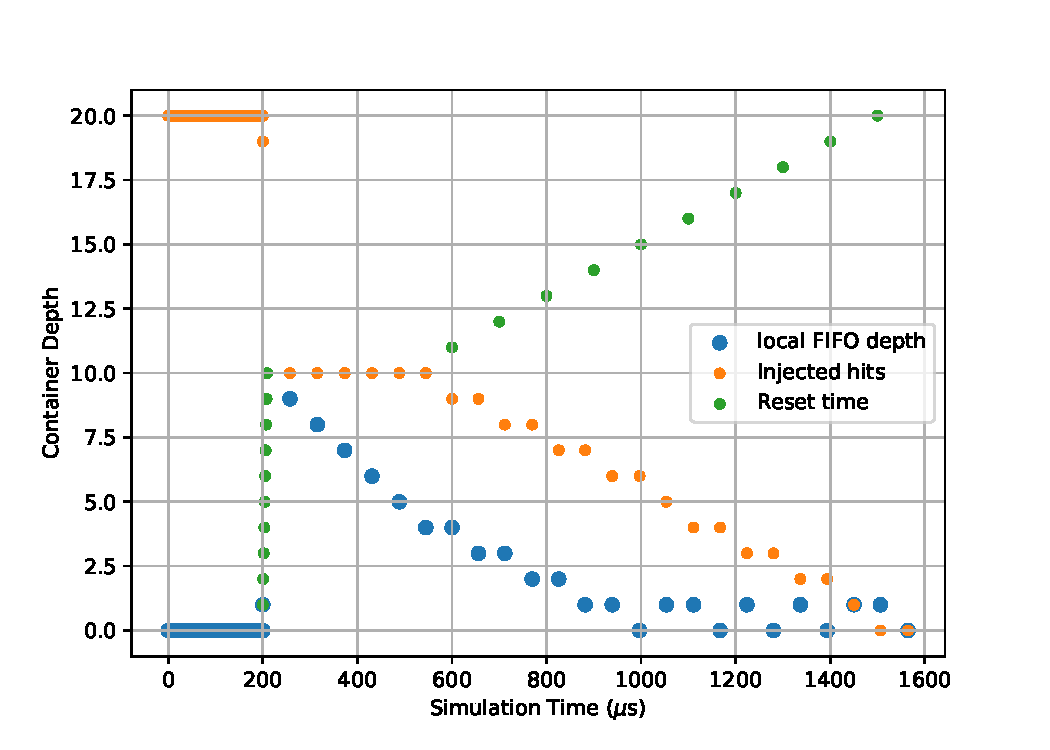
\includegraphics[width=\textwidth]{images/push_arch_buff.pdf}
\caption{A simulated push architecture with 20 injected hits at different times.
The time of the injected reset is indicated by the green points.
Before the simulation is run a node has its hits injected into a storage (orange) list.
Then, at each simulation time step ($\tau_{step}=1\unit{\mu s}$) the list is examined to see if a new hit will be written.
When a hit is found the relative time of the node can move forward in time to when this packet will be completed in time, while all other writes can occur to the local FIFO.
This is why the first local FIFO depth increases initially by one despite 10 nearly adjacent injected hits.
On the next time step, the depth then moves to nine; the simulation has sent the first of the 10 packets, and records nine.
This example correctly shows a maximum local FIFO depth of nine.
}
\end{figure}~\label{fig:push_arch_verification}